\documentclass[final,5p,times]{elsarticle}
\usepackage{iftex}
\ifPDFTeX
\usepackage[utf8]{inputenc}
\fi
\usepackage[T1]{fontenc}
\usepackage{amsmath}
\usepackage{amssymb}
\usepackage{multirow}
\usepackage{graphicx}
\usepackage{subcaption}
\usepackage{float}
\usepackage{tabularx}
\usepackage{microtype}
% Compatibility fallback for older LaTeX kernels that do not expose
% document-metadata conditionals expected by newer hyperref builds.
\makeatletter
\@ifundefined{IfDocumentMetadataTF}{\newcommand{\IfDocumentMetadataTF}[2]{#2}}{}
\@ifundefined{IfDocumentMetadataT}{\newcommand{\IfDocumentMetadataT}[1]{}}{}
\@ifundefined{IfDocumentMetadataF}{\newcommand{\IfDocumentMetadataF}[1]{#1}}{}
\makeatother
% \usepackage{svg} % Requires Inkscape for SVG integration
\newfloat{algorithm}{tbp}{loa}
\floatname{algorithm}{Algorithm}
\usepackage{tikz}
\usetikzlibrary{positioning, arrows.meta, fit, backgrounds, calc, shapes.geometric, decorations.pathmorphing}
\usepackage{algpseudocode}
\usepackage{hyperref}
\definecolor{ElsevierBlue}{RGB}{0,128,176}
\hypersetup{ colorlinks=true, linkcolor=ElsevierBlue, citecolor=ElsevierBlue, urlcolor=ElsevierBlue
}
% Keep bibliography entries from forcing narrow justified lines.
\makeatletter
\let\orig@thebibliography\thebibliography
\let\orig@endthebibliography\endthebibliography
\renewcommand{\thebibliography}[1]{%
  \orig@thebibliography{#1}%
  \raggedright
}
\renewcommand{\endthebibliography}{\orig@endthebibliography}
\makeatother
% ORCID support — renders as a clickable hyperlink in the PDF
\providecommand{\orcid}[1]{\texorpdfstring{\,\href{https://orcid.org/#1}{\textcolor{ElsevierBlue}{\small[ORCID:\,#1]}}}{ [ORCID: #1]}}
\makeatletter
\pdfstringdefDisableCommands{%
  \def\fnref#1{}%
  \def\corref#1{}%
  \def\@fnmark{}%
  \def\orcid#1{ [ORCID: #1]}%
  \def\textcolor#1#2{#2}%
  \def\small{}%
}
\makeatother
\journal{Swarm and Evolutionary Computation} % --- Symbols used in paper ---
\newcommand{\symStatedim}{\mathcal{D}_s}
\newcommand{\symActiondim}{\mathcal{D}_a}
\newcommand{\symPopsize}{N}
\newcommand{\symGamma}{\gamma}
\newcommand{\symMaxIters}{T_{\text{max}}}
\newcommand{\symBufferSize}{C_{\text{rb}}}
\newcommand{\symWindowsize}{W}
\newcommand{\symFeaturecount}{N_f}
\newcommand{\symHiddendimA}{H_a}
\newcommand{\symHiddendimB}{H_b}
\newcommand{\symBatchsize}{B}
\newcommand{\symLearningrate}{\eta}
\newcommand{\symNumepisodes}{E}
\newcommand{\symWarmup}{T_w}
\newcommand{\symNumruns}{N_{\text{runs}}}
\newcommand{\symRhoStag}{\rho_{\text{stag}}}
\newcommand{\symRhoCollapse}{\rho_{\text{coll}}}
\newcommand{\symRhoBonus}{\rho_{\text{div}}}
\newcommand{\symThetaMin}{\theta_{\min}}
\newcommand{\symKappaConv}{\kappa_{c}}
\newcommand{\symEtaCurios}{\eta_{u}}
\newcommand{\symUtd}{R_{\text{utd}}} 
% --- Adaptive Control Constants ---
\newcommand{\symExpInertia}{\kappa_w}
\newcommand{\symFeatWeightA}{\alpha_{f}}
\newcommand{\symFeatWeightB}{\beta_{f}}
\newcommand{\symResWeightW}{\eta_w}
\newcommand{\symResWeightC}{\eta_c}
\newcommand{\symWmaxSch}{w_{\max}}
\newcommand{\symWminSch}{w_{\min}}
\newcommand{\symCmaxSch}{c_{\max}}
\newcommand{\symCminSch}{c_{\min}}
\newcommand{\symWclipMin}{\underline{w}}
\newcommand{\symWclipMax}{\bar{w}}
\newcommand{\symCclipMin}{\underline{c}}
\newcommand{\symCclipMax}{\bar{c}}
\newcommand{\symThetaTol}{\epsilon_{\theta}}
\newcommand{\symScaleElite}{\omega_e}
\newcommand{\symStagMinGlobal}{\tau_{g,\min}}
\newcommand{\symStagRatioGlobal}{\mu_g}
\newcommand{\symStagMinPart}{\tau_{p,\min}}
\newcommand{\symStagRatioPart}{\mu_p}
\newcommand{\symStagMaxPart}{\tau_{\text{max}}}
\newcommand{\symSpread}{\eta_s}
\begin{document}
\begin{frontmatter}
\title{Soft Actor-Critic with Attractor-Field PSO Parameter Adaptation for UAV Path Planning}
\author[aff1]{Viet-Anh Ngo\orcid{0009-0002-5429-8554}}
\author[aff1]{Thanh-Hung Nguyen}
\ead{hung.nguyenthanh@hust.edu.vn}
\author[aff1,cor1]{Duc-Toan Nguyen}
\cortext[cor1]{Corresponding author}
\ead{toan.nguyenduc@hust.edu.vn}
\address[aff1]{School of Mechanical Engineering, Hanoi University of Science and Technology, 1A-Dai Co Viet Street, Bach Mai, Hanoi City, Viet Nam}
\begin{abstract}
Particle Swarm Optimization (PSO) is attractive for unmanned aerial vehicle (UAV) path planning because of its simplicity and fast convergence, but its performance remains highly sensitive to parameter selection.
This paper presents a Soft Actor-Critic (SAC)-guided PSO framework built around an attractor-field control law and a compact swarm-summary state.
The SAC agent is pretrained on a suite of standard benchmark functions before being deployed as a frozen policy on the target UAV planning problem.
A temporal-summary state encodes progress, diversity, feasibility, stagnation, and short-horizon trend information, while a scale-invariant relative-improvement reward keeps learning aligned with the optimization objective.
The core mechanism is a latent action that is expanded into particle-wise inertia, cognitive, and social coefficients through attractor-field modulation with geometric context signals, yielding structured heterogeneity without direct full per-particle control.
In a matched four-scenario study, the proposed attractor-field controller remains competitive with simpler control alternatives while preserving particle-wise variation without the action-space cost of direct per-particle control.
Across the benchmark, the compact-state SAC pipeline improves substantially over earlier frozen RL-based PSO baselines and remains competitive with strong adaptive PSO methods for UAV path planning.
These results indicate that both observation design and control-interface design materially affect pretrained SAC-guided PSO deployment.
\end{abstract}
\begin{keyword}
Particle Swarm Optimization \sep Soft Actor-Critic \sep UAV Path Planning \sep Adaptive Parameter Control \sep Swarm Intelligence \sep Attractor-Field Control
\end{keyword}
\end{frontmatter} 

\section{Introduction}
\label{sec:intro}
Unmanned Aerial Vehicles (UAVs) support missions ranging from precision agriculture to defense, disaster response \cite{Delavarpour2021A, Fascista2022Toward, Alotaibi2019LSAR}.
Every mission hinges on path planning to compute safe trajectories through cluttered three-dimensional environments.
Despite decades of study, planning in large, uncertain airspaces remains challenging because algorithms must simultaneously reason about vehicle dynamics, environmental constraints, and mission-specific trade-offs \cite{AitSaadi2022UAV, Zhou2025A}.
Recent work on coordinated missions highlights the complexity of multiobjective multi-UAV planning, where competing mission goals must be balanced under severe environmental constraints \cite{Meng2025Multiobjective}.

Among the many path planning methods, Particle Swarm Optimization (PSO) \cite{Kennedy1995Particle} has gained broad adoption for UAV path planning because of its conceptual simplicity, fast convergence, and natural fit for continuous search spaces \cite{Cheng2024Research}.
However, PSO's performance critically depends on carefully tuned inertia and acceleration coefficients, which are notoriously problem-dependent and can cause premature convergence when left static \cite{Yang2015Lowdiscrepancy}.
While adaptive PSO variants address this issue through feedback-driven or time-varying parameter schedules \cite{Bansal2011Inertia, Liu2025A}, such hand-designed rules often transfer poorly across terrains and obstacle densities and remain insensitive to changing swarm states.
Reinforcement learning (RL) offers a more principled alternative by treating parameter adaptation as a sequential decision problem.

Despite recent progress, RL-based PSO studies still leave one central question insufficiently resolved, namely whether performance gains come from the learning backbone itself or from how parameter control is distributed across the swarm.
Existing methods usually compare end-to-end designs that differ simultaneously in RL algorithm, state representation, reward formulation, and control interface, so the literature still lacks controlled evidence isolating the effect of control interface granularity under matched learning conditions.
Under that broader design mismatch, global control may be too coarse to reflect particle-level search status, fixed subgroup control imposes a predefined swarm structure, and direct per-particle control can greatly enlarge the action space and complicate learning.
Because prior comparisons usually mix these choices together, they do not support a clear causal account of whether gains come from the RL algorithm or from the control interface itself.
To address this gap, we propose AFSACPSO, a reinforcement-learning-guided PSO framework centered on a compact state representation and an attractor-field control law.
The paper makes three contributions. 
First, we introduces a lightweight temporal state of swarm progress, diversity, feasibility, stagnation, and short-horizon trend for frozen SAC-guided PSO deployment. 
Second, we proposes an attractor-field control law that expands a compact 9D latent action into particle-wise inertia, cognitive, and social coefficients using swarm context and particle rank, yielding structured heterogeneity without the action-space cost of direct per-particle control. 
Third, we evaluate these design choices under a matched protocol that separates external benchmark comparison from an internal same-backbone control-interface ablation and records the command path and artifact manifest needed to reproduce the reported tables and figures.

These contributions are evaluated in different ways.
The SAC agents are pretrained on a suite of 45 standard benchmark functions following the protocol of \cite{vonEschwege2024Soft}, then deployed as a frozen policy during evaluation, using the compact 15D swarm-summary state, a scale-invariant relative-improvement reward, twin critics, automatic entropy tuning, and target networks.
For external RL and classical benchmark comparisons, we use this SAC pipeline with the 15D state representation and report its strongest frozen deployment variant against RL-based and traditional self-adaptive baselines.
For the internal ablation, we compare global, fixed subgroup, direct per-particle, and attractor-field SAC control interfaces under the same SAC pipeline to isolate the attractor-field contribution itself.
Under that matched ablation, AFSACPSO remains competitive with the global controller while outperforming the fixed-subgroup and direct per-particle variants on the easier cases.
Against self-adaptive PSO variants, the current benchmark still shows lower mean fitness for SAEPSO in Scenarios 1 and 4 and for SAEPSO* in Scenarios 2 and 3 \cite{Liu2025A}, although it does not support a blanket runtime-speedup claim over the strongest classical baselines.
The remainder of this paper is organized as follows.
Section~\ref{sec:background} reviews PSO fundamentals and related adaptive strategies.
Section~\ref{sec:problem} formalizes the path planning problem.
Section~\ref{sec:methods} details the AFSACPSO architecture.
Section~\ref{sec:results} presents experimental results and supplementary training diagnostics.
Section~\ref{sec:discussion} discusses findings and outlines future directions.

\section{Related Work}
\label{sec:background} 
The UAV path planning literature is largely dominated by three paradigms: graph search, sampling-based approaches, and population-based optimization techniques \cite{AitSaadi2022UAV, Zhou2025A}.
Classical graph search methods such as A* and Dijkstra guarantee optimal paths on discretized maps \cite{Hart1968A}, but their cost scales poorly with map resolution and state dimensionality.
Sampling based planners such as RRT and PRM avoid explicit discretization and are attractive for high-dimensional path planning. In particular, RRT is well suited to non-holonomic and kinodynamic planning because it can explore the configuration space without requiring dense inter-state connections \cite{Karur2021A}.
Population based optimization remains attractive when the objective directly couples path length, terrain clearance, altitude, and obstacle avoidance.

Other population-based methods, including genetic algorithms, differential evolution, and Grey Wolf Optimizer, have also been applied successfully to UAV path planning under multi-constraint objectives \cite{Debnath2024An, AitSaadi2022UAV}.
Within this broader family, PSO is especially relevant here because it converges quickly in continuous search spaces and maps naturally to waypoint-based path parameterizations \cite{Cheng2024Research, Phung2021Safetyenhanced}.
Ensemble and self-adaptive PSO variants further improve robustness by varying search behaviors within the swarm \cite{Lynn2017Ensemble}, which makes PSO a suitable foundation for studying learned parameter adaptation.

Existing PSO adaptation strategies broadly fall into three groups: time-varying parameter schedules, feedback-driven adaptive schemes, and learning-based control methods.
Time-varying parameter schedules such as LDIW, TVAC, and oscillating or sinusoidal schedules are simple and computationally cheap \cite{Eberhart2000Comparing, Ratnaweera2004Selforganizing, Nickabadi2011A, Kentzoglanakis2009Particle, Chen2018A}.
These techniques have proven effective compared with many baselines, but they cannot react explicitly to swarm-specific stagnation or feasibility dynamics.
Feedback-driven adaptive schemes instead use online swarm feedback to dynamically adjust hyperparameters.
The SAEPSO algorithm of Liu et al. \cite{Liu2025A} adapts parameters on a per-particle basis through a normalized fitness-adaptation signal with sinusoidal temporal modulation.
UAPSO algorithm from Isiet et al. \cite{Isiet2019Selfadapting} derives its control parameters from an evolutionary state metric.
Both algorithms have shown superior performance compared with baseline algorithms on benchmark problems.
Adaptive state strategies such as APSO \cite{Zhan2009Adaptive} and entropy-based PSO variants \cite{Han2022Improved} likewise incorporate online search feedback, while fitness-adjusted parameter control has shown stronger benchmark performance than static schedules in prior studies \cite{Li2017Particle}.

Convergence analyses indicate that self-adaptation alone does not guarantee that PSO parameters remain within regions associated with stable convergence \cite{Harrison2018Selfadaptive}. 
This leaves open the critical question of how to adapt PSO parameters in a state-aware yet mathematically robust manner.
As an increasingly prevalent learning-based control method, reinforcement learning (RL) casts PSO parameter control as a sequential decision problem in which the controller observes swarm statistics, chooses parameter updates, and receives rewards tied to optimization progress \cite{Sutton2018Reinforcement, Bai2023Evolutionary}.
More broadly, RL-based control has also been studied in other population-based optimizers, including policy-gradient control in differential evolution and PPO-based parameter adaptation in iSOMA \cite{Sun2021Learning, Klein2024Optimizing}.

Across representative RL-PSO methods, the main design differences appear in how swarm information is encoded for the policy and in how parameter control is distributed across the swarm \cite{Meng2023Multistrategy, Aoun2024Deep, Li2023Reinforcement, Liu2023HRLPSO, Yin2023RLAMPSO, vonEschwege2024Soft}.
Value-based approaches typically discretize the action space and use RL for strategy selection rather than direct coefficient generation \cite{Watkins1992Qlearning}. 
In this line of work, the policy usually observes a coarse search-state description and selects from a predefined pool of PSO behaviors or update rules. MPSORL \cite{Meng2023Multistrategy}, for example, uses fitness-grade states to choose among hand-designed PSO strategies, DPQ-PSO \cite{Aoun2024Deep} combines DQN with Hidden Markov state inference, and RLNDM-PSO \cite{Li2023Reinforcement} classifies particles into four search states before switching among predefined velocity-generation behaviors. 
HRLPSO \cite{Liu2023HRLPSO} extends this general paradigm to a broader hybrid adaptation scheme. 
Taken together, these methods reduce the difficulty of continuous control, but they also tie performance to manually defined state abstractions and operator sets, which makes it difficult to disentangle the effect of the RL backbone from the effect of the chosen control interface.

\begin{table*}[htbp]
\centering
\small
\caption{Representative RL-based PSO parameter-control methods, organized by control granularity and state design. The comparison highlights that prior methods usually fix the control interface rather than compare control granularities under a matched RL backbone.}
\label{tab:rl_pso_comparison}
\resizebox{\textwidth}{!}{%
\begin{tabular}{lccccc}
\hline
Method & Control Granularity & RL Backbone & State & Reward & Notes \\
\hline
MPSORL \cite{Meng2023Multistrategy} & Discrete strategy & Q-Learning & fitness-grade snapshot & Fitness & strategy-pool selection \\
RLNDM-PSO \cite{Li2023Reinforcement} & Discrete strategy & Q-Learning & 4-state snapshot & Fitness & operator switching \\
DPQ-PSO \cite{Aoun2024Deep} & Discrete strategy & DQN & HMM+MLP & Fitness & target network \\
Wang et al. \cite{Wang2022ARL} & Discrete structural & Q-Learning & population-level counts & Fitness (relative) & level-based PSO topology \\
Zhang \& Chen \cite{Zhang2024ANovel} & Per-dimension discrete & Q-Learning & singular per-dimension & Hierarchical & per-dimension target selection \\
RLAM-PSO \cite{Yin2023RLAMPSO} & Fixed-subgroup continuous & DDPG & 3-stat snapshot & Fitness & group-specific coefficient triplets \\
HRLPSO \cite{Liu2023HRLPSO} & Hybrid continuous & Policy Grad. & MLP & Fitness & broader PSO adaptation \\
Diao et al. \cite{Diao2024An} & Offline seeding & SAC & system parameters & Euclidean dist. & teacher-student imitation \\
SAC-SAPSO \cite{vonEschwege2024Soft} & Global continuous & SAC & velocities + global stats & Fitness & 3D action shared by swarm \\
PPO-PSO \cite{Klein2024Optimizing} & Global continuous & PPO & swarm statistics & Fitness & online coefficient control \\
\hline
AFSACPSO (Ours) & Attractor-field particle-wise & SAC & 15D temporal summary & Fitness & 9D latent expansion \\
\hline
\end{tabular}%
}
\end{table*}

Other value based approaches use discrete actions to modify the swarm structure or target assignments.
Wang et al. \cite{Wang2022ARL} employ a discrete Q-learning approach to dynamically restructure a level-based PSO for large-scale optimization. 
By defining both the environment state and the action space as a predefined pool of discrete population level counts, the RL agent continuously adjusts the hierarchical depth of the swarm's learning topology. 
The Q-table is updated using a reward signal based on the relative fractional improvement of the global best fitness, enabling the algorithm to adaptively balance exploration and exploitation.
Zhang and Chen \cite{Zhang2024ANovel} implement a Q-learning framework to balance the symmetry between convergence and diversity by dynamically optimizing the learning targets of individual particles. 
In their approach, each dimension of every particle maintains a proprietary Q-table where the discrete action space consists of selecting which peer's personal best to learn from. 
The state space is singular for each dimension, and Q-values are updated using hierarchical rewards—awarding high payouts for global best improvements, moderate rewards for personal best updates, and penalties for stagnation.

Continuous control approaches replace discrete strategy selection with actor-critic adaptation.
RLAM-PSO \cite{Yin2023RLAMPSO} adapts PSO parameters dynamically using a Deep Deterministic Policy Gradient (DDPG) algorithm. 
It observes the environment through a three-feature snapshot state—consisting of iteration progress, spatial diversity, and no-improvement duration—which is expanded into a 15-dimensional state vector via sinusoidal transformations. 
By statically dividing the swarm into five subgroups, the continuous actor network emits a 20-dimensional action vector that maps directly into tailored inertia weights and acceleration coefficients for each group.
However, RLAM-PSO relies on an arbitrary, index-based static division of subgroups that assigns parameters unconditionally, ignoring the localized search contexts of individual particles.
Recent studies have also begun leveraging Soft Actor-Critic (SAC) architectures to handle continuous action spaces. Diao et al. \cite{Diao2024An} demonstrate the utility of such hybrid PSO-RL models for intelligent parameter identification in electrical power systems. 
Rather than continuously guiding particles during the optimization loop, they employ a teacher-student imitation learning framework where a Soft Actor-Critic (SAC) agent predicts a macro-level approximation of the model parameters. 
These predictions are then seeded as the initial population for a standard PSO algorithm, which fine-tunes the physical parameters to minimize the Euclidean distance between the simulated and actual active and reactive power outputs.
Eschwege and Engelbrecht \cite{vonEschwege2024Soft} adopt an entropy-regularized SAC architecture (SAC-SAPSO) to construct a self-adaptive controller. 
However, unlike decentralized multi-agent approaches, SAC-SAPSO employs a centralized agent that observes a concatenated environment state array, which comprises individual particle velocities alongside macroscopic swarm metrics like the aggregate percentages of stable and infeasible particles. 
This single centralized RL agent then emits exactly one shared 3D continuous action vector containing the inertia weight and acceleration coefficients ($w, c_1, c_2$), which acts as the single global configuration for the entire swarm simultaneously.

Taken together, this literature demonstrates rapid evolution in RL backbones transitioning from discrete action selection to advanced continuous action frameworks, but offers surprisingly weak causal evidence regarding control interface design. 
Prior studies inherently commit to a single structural interface a priori, whether that entails decentralized multi-agent discrete selection, static continuous subgroup partitioning, single global parameter broadcasting, or offline imitation seeding—and then evaluate their algorithm's end-to-end performance against models that simultaneously differ in their state formulations, RL backbones, and reward structures. 
Consequently, the literature yields virtually no controlled ablation evidence isolating how the spatial granularity of control itself impacts optimization outcomes under a fixed RL architecture. 
While state representation and reward engineering undoubtedly govern agent behavior, the principal unresolved structural question is whether macroscopic global tuning, static subgroup partitioning, or high-dimensional direct particle-wise continuous action distribution actually serves as the optimal control interface for RL-driven phase-space exploration. 
Table~\ref{tab:rl_pso_comparison} maps representative RL-PSO methodologies against these architectural axes and situates AFSACPSO within the broader design space.

\section{Problem Formulation}
\label{sec:problem}
The UAV path planning problem formulation and fitness objective presented in this section were developed based on the framework established in \cite{Liu2025A}.
We address the problem of planning a collision-free trajectory for a UAV operating in a 3D airspace.
The environment is represented by a digital elevation map (DEM) $\mathcal{E}: \mathbb{R}^2 \to \mathbb{R}$ that returns terrain height for any $(x, y)$ coordinate, augmented with a set of cylindrical no-fly zones $\mathcal{O} = \{(c_j, r_j, h_j)\}_{j=1}^{M}$ representing threat areas.
The UAV must navigate from a start position $s_{\text{start}} \in \mathbb{R}^3$ to a goal position $s_{\text{goal}} \in \mathbb{R}^3$ while minimizing the fitness function defined in Equation~\ref{eq:fitness}.
\begin{figure}[!htb]
\centering
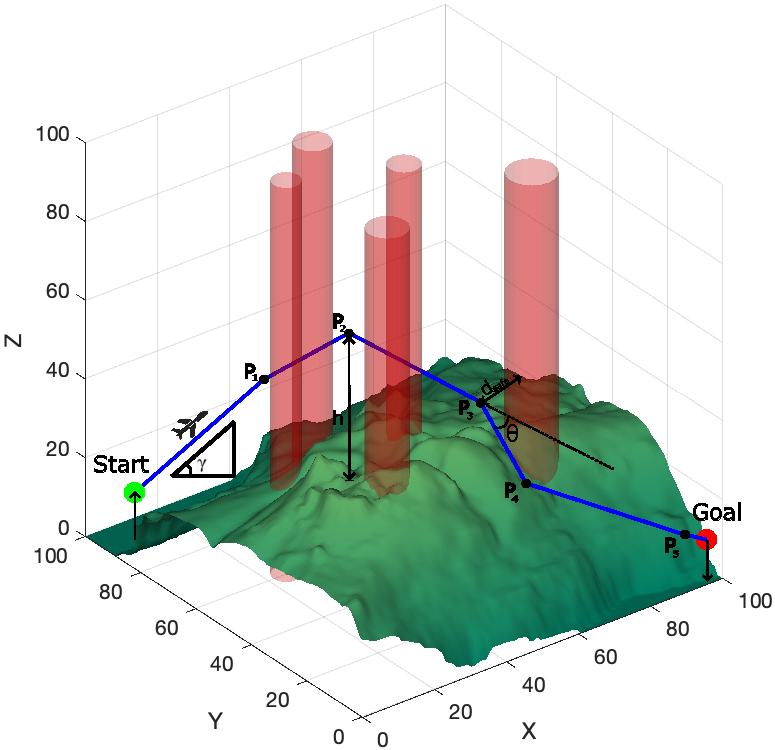
\includegraphics[width=\linewidth]{data/ProblemFormulation.pdf}
\caption{Geometric definition of UAV path planning parameters}
\label{fig:problem_formulation}
\end{figure}
A candidate path is encoded as a sequence of $n$ waypoints $P = [p_1, p_2, \ldots, p_n]$ where each $p_i = (x_i, y_i, z_i) \in \mathbb{R}^3$.
The UAV follows linear segments between consecutive waypoints, yielding total path length
\begin{equation}
L(P) = \sum_{i=1}^{n-1} \|p_{i+1} - p_i\|_2
\label{eq:path_length}
\end{equation}
Path quality is evaluated through a weighted fitness function that balances competing objectives
\begin{equation}
\begin{aligned}
f(P) ={}& \lambda_1 L(P) + \lambda_2 C_{\text{turn}}(P) + \lambda_3 C_{\text{climb}}(P) \\
&+ \lambda_4 C_{\text{alt}}(P) + C_{\text{safety}}(P)
\end{aligned}
\label{eq:fitness}
\end{equation}
The turn penalty $C_{\text{turn}}$ applies a linear penalty for directional changes that exceed a minimal tolerance threshold
\begin{equation}
C_{\text{turn}}(P) = \sum_{i=2}^{n-1} \max\left(0, \theta_i - \theta_{\max}\right)
\end{equation}
where $\theta_i$ is the turn angle between consecutive segments $i-1$ and $i$, and $\theta_{\max}$ is the maximum zero-penalty turn threshold (set to $\symThetaTol$ rad).
The climb penalty $C_{\text{climb}}$ penalizes both steep climb adjustments and absolute climb angles
\begin{equation}
\begin{aligned}
C_{\text{climb}}(P) = \sum_{i=2}^{n-1} \left( 2|\xi_i - \xi_{i-1}| + |\xi_i| + |\xi_{i-1}| \right)
\end{aligned}
\end{equation}
where $\xi_i = \arctan\left(\frac{z_{i+1} - z_i}{\|p_{i+1} - p_i\|_{xy}}\right)$ is the climb angle of the $i$-th segment. The safety penalty $C_{\text{safety}}$ acts as an absolute constraint combining terrain, obstacle, and path feasibility violations (applying infinite or heavy penalties for penetrating restricted boundaries) and is defined as
\begin{equation}
\begin{aligned}
C_{\text{safety}}(P) = \sum_{i=1}^{n} \Bigl[ &\max(0, \mathcal{E}(x_i, y_i) + h_{\min} - z_i) \\
&+ \sum_{j=1}^{M} \max(0, r_j - d_{ij}) \Bigr]
\end{aligned}
\end{equation}
where $d_{ij}$ is the distance from waypoint $i$ to obstacle $j$.
The altitude cost $C_{\text{alt}}$ encourages the UAV to maintain low-level flight for terrain masking and energy efficiency
\begin{equation}
C_{\text{alt}}(P) = \sum_{i=1}^{n} z_i
\end{equation}
The normalized weights $\lambda_1, \ldots, \lambda_4$ balance efficiency against soft constraints.
The safety term $C_{\text{safety}}$ dominates the objective to enforce strict feasibility.
Lower fitness values indicate better paths.

\section{Methods}
\label{sec:methods}
The RL-based PSO parameter adaptation problem is formulated as a Markov Decision Process (MDP).
In the proposed algorithm, the MDP is defined by the tuple $(\mathcal{S}, \mathcal{A}, \mathcal{R}, \mathcal{T}, \symGamma)$ as illustrated in Figure~\ref{fig:mdp_components}.
The state space $\mathcal{S}$ encodes compact swarm statistics over a short temporal window.
The action space $\mathcal{A}$ is a $\symActiondim$-D latent control vector which is expanded into particle-wise PSO coefficients through the attractor-field parameter expansion.
The reward function $\mathcal{R}$ provides scale-invariant feedback from the relative improvement in global best fitness.
The transition rules $\mathcal{T}$ describe deterministic updates computed via the standard PSO velocity and position equations, functioning effectively as the environment transition function during learning.
The discount factor $\symGamma$ determines the temporal preference for cumulative returns.
\begin{figure*}[!t]
\centering
\resizebox{\textwidth}{!}{%
\begin{tikzpicture}[
    x=1cm,
    y=1cm,
    >=Stealth,
    font=\normalsize,
    panel/.style={
        draw=black!35,
        thick,
        rounded corners=12pt,
        inner sep=14pt
    },
    box/.style={
        draw=black!65,
        thick,
        rounded corners=8pt,
        fill=white,
        align=center,
        inner sep=5pt,
        minimum height=2.2cm
    },
    smallbox/.style={
        draw=black!60,
        thick,
        rounded corners=7pt,
        fill=white,
        align=center,
        inner sep=4pt,
        minimum height=1.5cm
    },
    flow/.style={draw=black!80, line width=1.1pt, ->},
    train/.style={draw=red!70!black, line width=1.0pt, dashed, ->},
    faint/.style={draw=black!40, line width=0.9pt, ->},
    note/.style={
        draw=black!45,
        rounded corners=6pt,
        fill=yellow!12,
        align=center,
        font=\small,
        inner sep=4pt
    }
]

% Agent-side illustrations (x positions tightened for better aspect after \resizebox)
\node[box, fill=blue!7, minimum width=7.4cm, inner sep=6pt, yshift=-8pt, align=center] (state_enc) at (-4.2, -0.02) {%
\textbf{State Encoder}\\[0.2em]
\begin{tikzpicture}[scale=0.95]
    \useasboundingbox (-3.7, -1.2) rectangle (3.7, 1.2);
    
    % --- History Scope ---
    \begin{scope}[xshift=-1.9cm]
        \node[font=\small\bfseries, text=black!80, anchor=south] at (0.1, 0.85) {Swarm History};
        \draw[black!20, line width=0.4pt, dashed] (1.2, 0.75) -- (1.2, -0.9);
        \foreach \i in {1,...,9} {
            \pgfmathsetmacro{\y}{(5 - \i)*0.18}
            \draw[black!15, line width=0.3pt] (-1.0, \y) -- (1.2, \y);
            \draw[blue!55, line width=0.65pt, smooth, samples=20, domain=-1.0:1.2]
                plot (\x, { \y + 0.05*sin(\x*160 + \i*50) + 0.02*cos(\x*280 - \i*20) + 0.02*\x*sin(\i*110) });
            \pgfmathsetmacro{\cy}{\y + 0.05*sin(1.2*160 + \i*50) + 0.02*cos(1.2*280 - \i*20) + 0.02*1.2*sin(\i*110)}
            \fill[blue!80!black] (1.2, \cy) circle (0.8pt);
        }
        % Vertical axis for features
        \draw[-{Stealth[length=1.2mm]}, black!35, line width=0.4pt] (-1.15, -0.9) -- (-1.15, 0.75) 
            node[pos=0.5, above, sloped, font=\fontsize{5}{6}\selectfont, text=black!60, inner sep=2pt] {features};
        \draw[-{Stealth[length=1.2mm]}, black!35, line width=0.4pt]
            (-1.15, -0.9) -- (1.2, -0.9) node[pos=0.5, below, font=\fontsize{5}{6}\selectfont, text=black!60, inner sep=2pt] {$W$ (time)};
    \end{scope}
    
    % --- Extraction Arrow ---
    \draw[-{Stealth[length=1.5mm]}, black!50, line width=0.8pt] (-0.4, 0) -- (0.4, 0); 
        
    % --- State Scope ---
    \begin{scope}[xshift=1.9cm]
        \node[font=\small\bfseries, text=black!80, anchor=south] at (0, 0.85) {Swarm's State};
        
        % Group 1: Current (9)
        \foreach \i in {0,...,8} {
            \draw[draw=blue!55, fill=blue!12, rounded corners=0.5pt] (-1.26 + \i*0.16, -0.15) rectangle +(0.14, 0.35);
        }
        
        % Group 2: Mean (3)
        \foreach \i in {0,...,2} {
            \draw[draw=teal!55, fill=teal!12, rounded corners=0.5pt] (0.24 + \i*0.16, -0.15) rectangle +(0.14, 0.35);
        }
        
        % Group 3: Trend (3)
        \foreach \i in {0,...,2} {
            \draw[draw=violet!55, fill=violet!12, rounded corners=0.5pt] (0.78 + \i*0.16, -0.15) rectangle +(0.14, 0.35);
        }
    \end{scope}
\end{tikzpicture}};

\node[box, fill=orange!10, minimum width=5.35cm, minimum height=0pt, inner xsep=4.5pt, inner ysep=12pt, yshift=-8pt, text width=\dimexpr5.35cm-9pt\relax, align=center] (sac) at (3.05, -0.02) {%
\textbf{SAC Controller}\\[0.35ex]%
\begin{tikzpicture}[scale=1.845]
\begin{scope}[xshift=-0.32cm]
% text width on parent node: title and inner picture share the same horizontal center
    \coordinate (sacxl) at (0.00,0);
    \coordinate (sacxr) at (1.67,0);
    % ---- Actor (upper)
    \node[font=\small\bfseries, text=blue!70!black, yshift=18pt] at ($(sacxl)!0.5!(sacxr)+(0,0.87)$) {Actor};
    \foreach \y in {0.42,0.62,0.82} \fill[green!45!black] (0.0,\y) circle (2.7pt);
    \foreach \y in {0.32,0.52,0.72,0.92} \fill[gray!65] (0.86,\y) circle (2.7pt);
    \foreach \a in {0.32,0.52,0.72,0.92} \draw[gray!45] (0.02,0.42) -- (0.84,\a);
    \foreach \a in {0.32,0.52,0.72,0.92} \draw[gray!45] (0.02,0.62) -- (0.84,\a);
    \foreach \a in {0.32,0.52,0.72,0.92} \draw[gray!45] (0.02,0.82) -- (0.84,\a);
    \fill[orange!70] (1.67,0.62) circle (3.45pt);
    \foreach \a in {0.32,0.52,0.72,0.92} \draw[orange!60] (0.88,\a) -- (1.65,0.62);
    % ---- Twin $Q$ as two mirrored critic networks
    \foreach \x/\label in {0.34/$Q_{\phi_1}$,1.18/$Q_{\phi_2}$} {
        \foreach \y in {-0.18,-0.43,-0.68} \fill[green!45!black] (\x-0.24,\y) circle (2.5pt);
        \foreach \y in {-0.18,-0.43,-0.68} \fill[gray!65] (\x,\y) circle (2.5pt);
        \foreach \a in {-0.18,-0.43,-0.68} \draw[gray!45] (\x-0.22,-0.18) -- (\x-0.02,\a);
        \foreach \a in {-0.18,-0.43,-0.68} \draw[gray!45] (\x-0.22,-0.43) -- (\x-0.02,\a);
        \foreach \a in {-0.18,-0.43,-0.68} \draw[gray!45] (\x-0.22,-0.68) -- (\x-0.02,\a);
        \fill[red!72] (\x+0.24,-0.43) circle (3.0pt);
        \foreach \a in {-0.18,-0.43,-0.68} \draw[red!58] (\x+0.02,\a) -- (\x+0.22,-0.43);
        \node[font=\scriptsize, text=red!85!black, anchor=north] at (\x+0.24,-0.54) {\label};
        \draw[orange!55, dashed, line width=0.45pt] (1.67,0.70) -- (\x+0.24,-0.28);
    }
    \node[font=\small\bfseries, text=red!72!black, anchor=south, inner sep=0.3pt, outer sep=0pt] at ($(sacxl)!0.5!(sacxr)+(0,0.048)$) {Twin $Q$};
\end{scope}
\end{tikzpicture}};

\node[smallbox, fill=orange!14, minimum width=2.7cm, yshift=-8pt] (action) at (9.15, -0.02) {%
\textbf{Latent Action}\\[0.12em]
\begin{tikzpicture}[scale=0.85]
    \useasboundingbox (-1.25, -0.1) rectangle (1.25, 0.8);
    \draw[black!32, line width=0.4pt] (-1.15,0) -- (1.15,0);
    \foreach \i in {0,...,8} {
        \pgfmathsetmacro{\x}{(\i - 4)*0.24}
        \pgfmathsetmacro{\h}{0.18 + 0.52*abs(cos(\i*31+7))}
        \fill[orange!78!black, rounded corners=0.5pt] (\x-0.08, 0) rectangle (\x+0.08, \h);
    }
\end{tikzpicture}};

\node[smallbox, fill=red!7, minimum width=2.9cm] (replay) at (13.55, -1.35) {%
\textbf{Replay Buffer}};

% Environment-side illustrations
\node[box, fill=yellow!12, minimum width=3.4cm] (reward) at (-7.85, -6.35) {%
\textbf{Relative Reward}\\[0.1em]
\begin{tikzpicture}[scale=1.1]
    \draw[draw=black!40, ->] (0,0) -- (1.8,0);
    \draw[draw=black!40, ->] (0,0) -- (0,1.2);
    \clip (0,0) rectangle (1.8,1.2);
    \draw[samples=50, domain=0:1.5, line width=1.3pt, green!65!black] plot (\x, {0.15*\x + 0.3*sin(2.5*\x r)});
    \node[font=\scriptsize] at (0.9,-0.3) {$\mathcal{R}(f_{t-1},f_t)$};
\end{tikzpicture}};

\node[box, fill=green!8, minimum width=3.4cm, inner sep=0pt] (eval) at (-3.05, -6.35) {%
\textbf{Fitness \& Swarm Stats}\\[0.1em]
\begin{tikzpicture}
    \node[blend mode=multiply, inner sep=0pt] {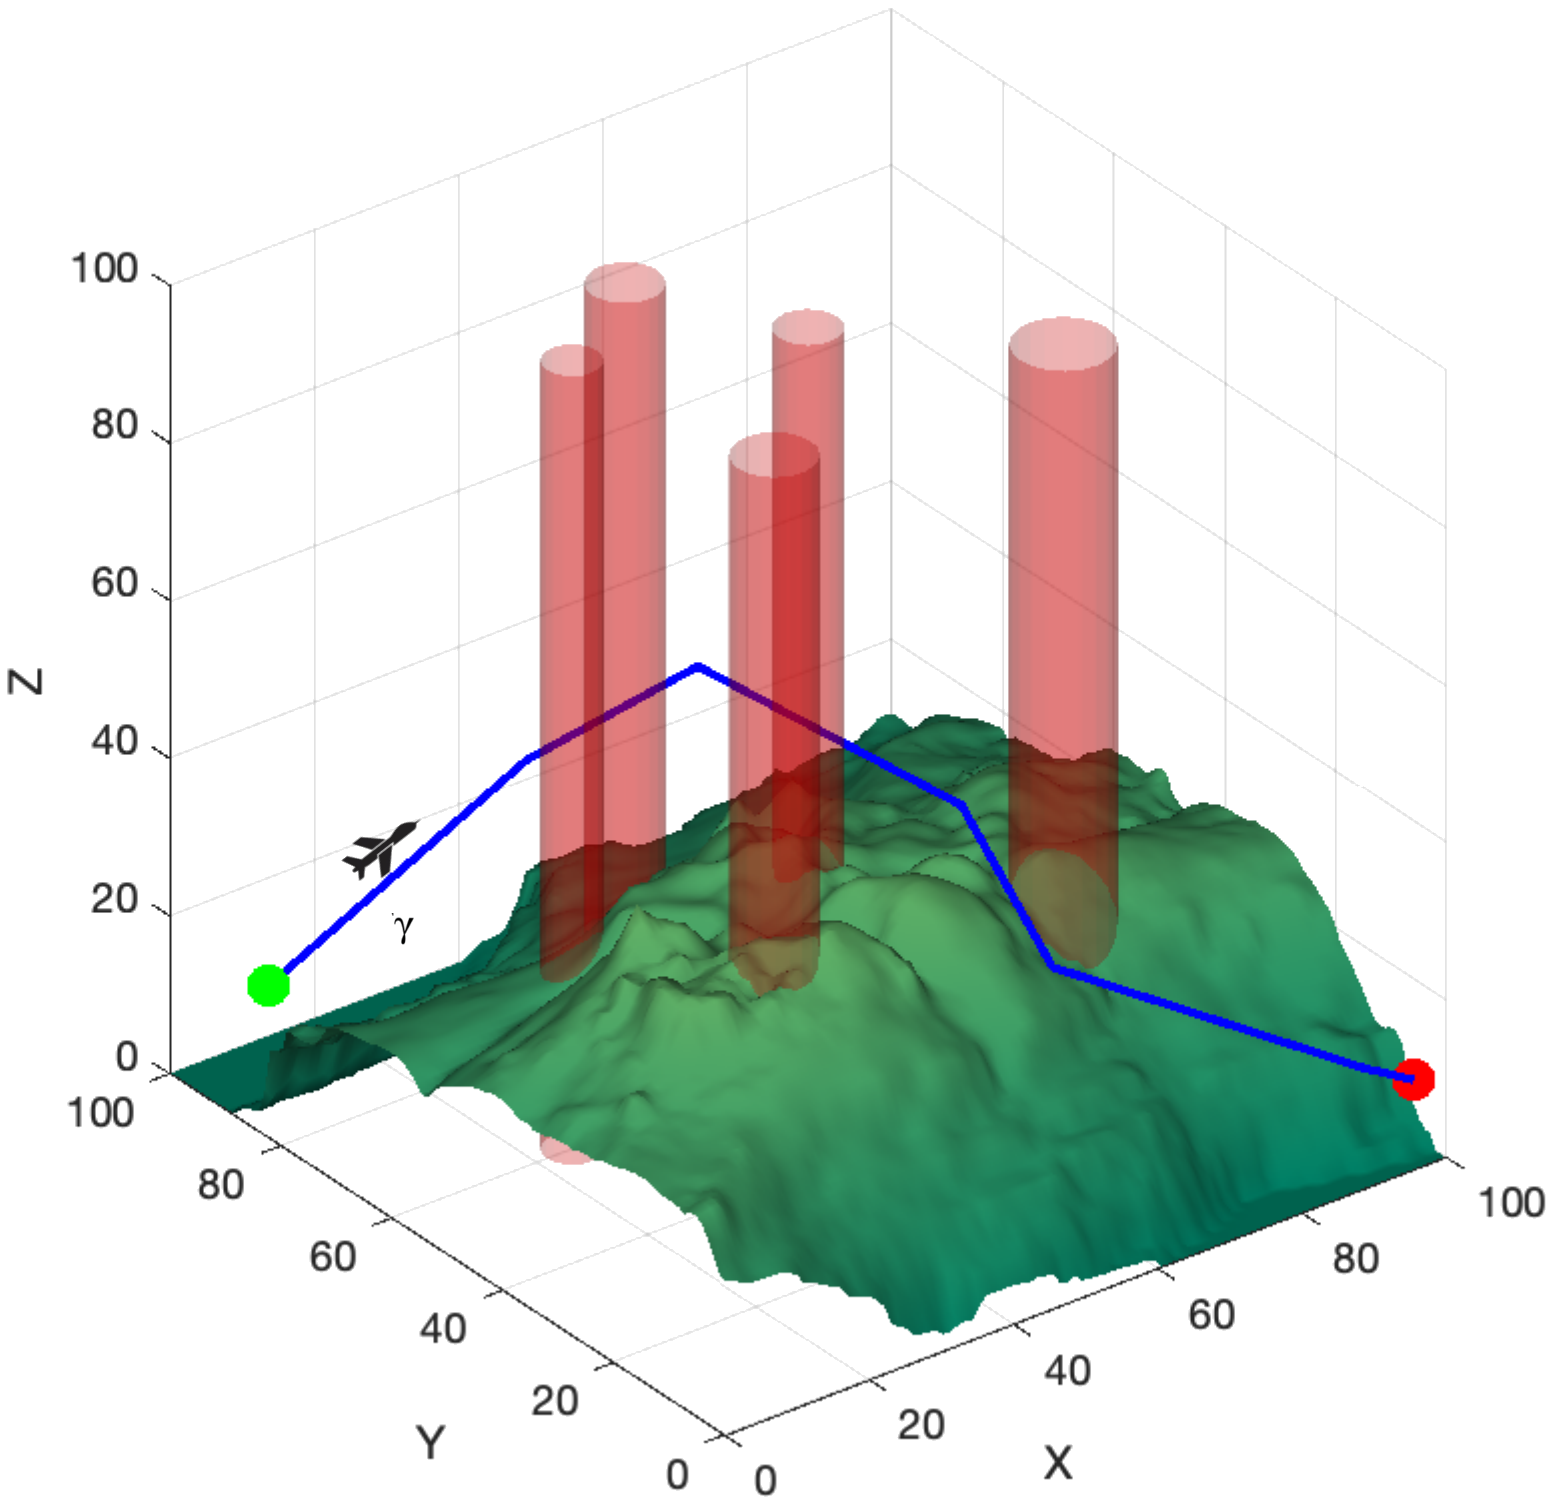
\includegraphics[width=3.4cm, trim=0 0.8cm 0 0.5cm, clip]{data/extracted_image.png}};
\end{tikzpicture}};

\node[box, fill=green!8, minimum width=4.0cm] (swarm) at (3.05, -6.35) {%
\textbf{PSO Search Step}\\[-0.15em]
\begin{tikzpicture}[scale=0.86]
    % Nature-based landscape (faint contours)
    \foreach \r in {0.4, 0.8, 1.2} \draw[black!8, decoration={random steps, segment length=3mm, amplitude=0.4pt}, decorate] (1.6, 0.6) ellipse (\r*1.1 cm and \r*0.5 cm);
    
    \foreach \i in {1,...,24} {
        \pgfmathsetmacro{\tx}{rnd*2.6 + 0.2}
        \pgfmathsetmacro{\ty}{rnd*0.8 + 0.15}
        \pgfmathsetmacro{\ang}{rnd*360}
        \pgfmathsetmacro{\dist}{rnd*0.25 + 0.15}
        \pgfmathsetmacro{\dx}{\tx + \dist*cos(\ang)}
        \pgfmathsetmacro{\dy}{\ty + \dist*sin(\ang)}
        \pgfmathsetmacro{\clrindex}{int(mod(\i,6))}
        \ifcase\clrindex
          \def\c{teal}\or\def\c{olive}\or\def\c{violet}\or\def\c{cyan!80!black}\or\def\c{orange!90!black}\or\def\c{red!70!black}\fi
        % Motion trail
        \draw[\c!30, line width=0.8pt, line cap=round] (\tx,\ty) -- (\dx,\dy);
        % Start pos (soft fade)
        \fill[\c!20] (\tx,\ty) circle (1.1pt);
        % Particle (solid)
        \fill[\c!85] (\dx,\dy) circle (1.6pt);
        % Micro-vector header
        \draw[\c!95, -{Stealth[scale=0.4]}] (\dx,\dy) -- ++(\ang:0.1);
    }
    % apply coefficients and gbest removed
\end{tikzpicture}};

\node[box, fill=orange!10, minimum width=3.5cm] (expand) at (9.15, -6.35) {%
\textbf{Attractor-Field Expansion}\\[-0.15em]
\begin{tikzpicture}[scale=0.85]
    \foreach \r in {0.25,0.5,0.75} \draw[orange!35] (0,0) circle (\r);
    \fill[orange!75] (0,0) circle (2.4pt);
    \node[font=\scriptsize\bfseries] at (0,0.28) {$a_t$};
    \draw[draw=blue!55, fill=blue!10, rounded corners=4pt] (0.55,0.55) rectangle +(1.0,0.22);
    \draw[draw=blue!55, fill=blue!10, rounded corners=4pt] (0.55,0.15) rectangle +(1.0,0.22);
    \draw[draw=blue!55, fill=blue!10, rounded corners=4pt] (0.55,-0.25) rectangle +(1.0,0.22);
    \node[font=\scriptsize] at (1.05,0.66) {$w_i$};
    \node[font=\scriptsize] at (1.05,0.26) {$c_{1,i}$};
    \node[font=\scriptsize] at (1.05,-0.14) {$c_{2,i}$};
    \draw[faint] (0.08,0.02) -- (0.55,0.66);
    \draw[faint] (0.08,0.00) -- (0.55,0.26);
    \draw[faint] (0.08,-0.02) -- (0.55,-0.14);
    \node[font=\scriptsize] at (0.72,-0.58) {particle-wise coefficients};
\end{tikzpicture}};

\node[smallbox, fill=yellow!10, minimum width=2.6cm] (context) at (13.55, -6.35) {%
\textbf{Context}\\
\small rank + geometry\\
modulation};

% Background panels
\begin{scope}[on background layer]
    \node[panel, fill=blue!4, fit=(state_enc)(sac)(action)(replay), inner xsep=12pt, inner ysep=6pt] {};
    \node[font=\Large\bfseries] at (1.2, 3.25) {Agent (SAC controller)};

    \node[panel, fill=green!4, fit=(reward)(eval)(swarm)(expand)(context), inner xsep=12pt, inner ysep=5pt] {};
    \node[font=\Large\bfseries] at (1.2, -4.05) {Environment};
\end{scope}

% Main loop
\draw[flow] (state_enc) -- node[above, font=\small] {$s_t \in \mathbb{R}^{15}$} (sac);
\draw[flow] (sac) -- node[above, font=\small] {policy output} (action);
\draw[flow] (action) -- node[right, pos=0.6, font=\small] {$a_t \in \mathbb{R}^{9}$} (expand);
\draw[flow] (context) -- (expand);
\draw[flow] (expand) -- node[above, font=\small] {$w_i,\ c_{1,i},\ c_{2,i}$} (swarm);
\draw[flow] (swarm) -- node[above, font=\small] {updated particles} (eval);
\draw[flow] (eval.north) -- node[right, font=\small] {9 swarm features $f_{1:9}$} (eval.north |- state_enc.south);
\draw[flow] (eval) -- node[above, font=\small] {$r_t$} (reward);

% Training-only loop: $s_t$ into replay (south $\rightarrow$ south; two right-angle turns)
\draw[train, rounded corners=10pt] (state_enc.south) -- ++(0,-2.35cm) -| (replay.south);
% Simplified 1-turn transition path from mid-east
\draw[train, rounded corners=10pt] ([yshift=1.35cm]sac.east) -| (replay.north);
\draw[train, rounded corners=10pt] (reward.north) -- ++(0, 2.0cm) -| (replay.south);
% transitions label removed



\end{tikzpicture}%
}
\caption{MDP/data-flow view of the AFSACPSO configuration}
\label{fig:mdp_components}
\end{figure*}

The method described in this section refers to the AFSACPSO pipeline, which combines the compact 15D swarm-summary state with the attractor-field control interface. Relative to the earlier SAC-SAPSO-style observation design, the pipeline first changes what information is presented to the SAC controller and then changes how the learned action is distributed across particles.
To address the limitations of static state observations used in prior RL-PSO methods, we adopt a compact swarm-statistics state representation. This follows state-representation literature, which treats the state as a compact depiction of observations that preserves the information necessary for control and often benefits from temporal continuity or predictive dynamics \cite{Lesort2018State}.
At each iteration, the controller extracts nine normalized swarm-level features $f_1, \dots, f_9 \in [0,1]$ summarizing progress, diversity, fitness, constraints, and swarm kinematics. The exact mathematical formulation for each feature is detailed in Table~\ref{tab:state_features}.

\begin{table*}[htbp]
\centering
\small
\caption{Mathematical formulation of the 9 normalized swarm-level features }
\label{tab:state_features}
\renewcommand{\arraystretch}{1.3}
\begin{tabular}{llp{9.2cm}}
\hline
\textbf{Feature} & \textbf{Formula} & \textbf{Description} \\
\hline
$f_1$ Iteration progress & $t / \symMaxIters$ & Linear fraction of the search budget consumed. \\
$f_2$ Spatial diversity ratio & $\frac{1}{D} \sum_{d=1}^D \frac{\sigma(x_{\cdot,d})}{\Delta_d + \epsilon}$ & Average ratio of population standard deviation to bounding box span per dimension. \\
$f_3$ Elite fitness advantage & $\tanh\left(\symScaleElite \frac{\operatorname{median}(F) - \min(F)}{|\operatorname{median}(F)| + \epsilon}\right)$ & Normalized gap between median and best fitness, mapping large gaps asymptotically to 1. \\
$f_4$ Global stagnation & $\min\left(1, \frac{t - t_{\text{last\_improve}}}{\max(\symStagMinGlobal, \symStagRatioGlobal \symMaxIters)}\right)$ & Normalized iterations since the last global fitness improvement. \\
$f_5$ Feasibility-quality & $\symFeatWeightA \mu_{\text{feas}} + \symFeatWeightB \frac{1}{1 + \ln(1 + f_{\text{gbest}})}$ & Weighted combination of the feasible-particle ratio ($\mu_{\text{feas}}$) and log-scaled global best fitness. \\
$f_6$ Constraint-pressure & $\min(1, \mu_{\text{coll}} + P_{\text{terrain}} + P_{\text{danger}} + P_{\text{dup}})$ & Sum of collision ratio and log-scaled penalty averages ($P_k$) for terrain, danger zones, and duplicates. \\
$f_7$ Global-best attraction & $1 - \tanh\left(\frac{\frac{1}{\symPopsize}\sum_i \|x_i - g\|_2}{\bar{\Delta}\sqrt{D} + \epsilon}\right)$ & Inverse of the average distance to the global best relative to the expected bounding box diagonal. \\
$f_8$ Velocity alignment & $0.5 + 0.5 \left( \frac{1}{\symPopsize}\sum_i \frac{v_i \cdot (g - x_i)}{\|v_i\|_2 \|g - x_i\|_2 + \epsilon} \right)$ & Average cosine similarity between particle velocities and the direction to the global best. \\
$f_9$ Particle stagnation & $\frac{1}{\symPopsize} \sum_i \min\left( \frac{s_i}{\max(\symStagMinPart, \symStagRatioPart \symMaxIters)}, 1 \right)$ & Average normalized individual stagnation counter $s_i$ (iterations since personal best improved). \\
\hline
\end{tabular}
\end{table*}

These features are buffered over a temporal window of $\symWindowsize$ iterations.
In the benchmarked setup, the deployed encoder is intentionally lightweight. It forms a $\symStatedim$-D state by concatenating the current nine features, the first three coordinates of the temporal mean, and the first three coordinates of the one-step trend.
This keeps the controller lightweight while still exposing short-horizon temporal context.
The nine base swarm features are clipped to $[0,1]$ before temporal aggregation. The appended trend terms in the final 15D state may be signed.
In the mathematical formulations detailed in Table~\ref{tab:state_features}, let $x_{i,d}$ and $v_{i}$ denote the position and velocity of particle $i$, $g$ the global best position, $F$ the set of valid particle fitnesses, $\symMaxIters$ the maximum iterations, $\symPopsize$ the swarm size, $D$ the problem dimension, and $\Delta_d = \max_i x_{i,d} - \min_i x_{i,d}$.
Table~\ref{tab:state_features} summarizes the feature design at the method level. The implementation uses fixed constants for the normalizers and weights in the corresponding code path.

The controller uses a scale-invariant relative improvement reward following \cite{vonEschwege2024Soft}. Let $f^{t-1}$ and $f^{t}$ denote the global best fitness before and after the PSO update at iteration $t$. The reward is
\begin{equation}
r_t = \frac{2\left(f^{t-1} - f^{t}\right)}{\left|f^{t-1}\right| + \left|f^{t}\right| + \epsilon}
\label{eq:reward_total}
\end{equation}
where $\epsilon = 10^{-8}$ prevents division by zero.
This formulation is bounded in $[-2, 2]$, positive when fitness improves, negative when it worsens, and zero when unchanged. Because it normalizes by the absolute fitness values, the reward magnitude is consistent across functions with different fitness scales, which is essential for pretraining across diverse benchmark landscapes.

AFSACPSO employs Soft Actor-Critic \cite{Haarnoja2018Soft} to learn the parameter-adaptation policy.
The SAC objective is the entropy-regularized expected return
\begin{equation}
J(\pi) = \mathbb{E}_{\tau \sim \pi}\left[\sum_{t=0}^{T} \gamma^t \left(r_t + \alpha \mathcal{H}(\pi(\cdot|\mathbf{s}_t))\right)\right]
\label{eq:sac_objective}
\end{equation} where $\alpha$ is the temperature parameter (automatically tuned) and $\mathcal{H}$ is the policy entropy.
The algorithm maintains three components. The actor network $\pi_\theta(\mathbf{a}|\mathbf{s})$ is a Gaussian policy with learnable mean and diagonal covariance. In our implementation the actor is a compact MLP operating on the flat 15D state vector. Actions are sampled via reparameterization as
\begin{equation}
\mathbf{a}_t = \tanh(\boldsymbol{\mu}_\theta(\mathbf{s}_t) + \boldsymbol{\sigma}_\theta(\mathbf{s}_t) \odot \boldsymbol{\epsilon}), \quad \boldsymbol{\epsilon} \sim \mathcal{N}(0, \mathbf{I})
\end{equation} The twin critic networks $Q_{\phi_1}$ and $Q_{\phi_2}$ are two independent scalar Q-functions used together with target networks. The critic loss minimizes the Bellman error using the minimum of both critics as
\begin{equation}
\begin{aligned}
L_Q(\phi_i) = \mathbb{E}_{(\mathbf{s},\mathbf{a},r,\mathbf{s}')} \Bigl[ \bigl(Q_{\phi_i}(\mathbf{s}, \mathbf{a}) - (&r + \symGamma \min_{j=1,2} Q_{\phi_j}(\mathbf{s}', \mathbf{a}') \\
&- \alpha \log \pi_\theta(\mathbf{a}'|\mathbf{s}') )\bigr)^2 \Bigr]
\end{aligned}
\end{equation} The temperature parameter $\alpha$ is automatically adjusted to match a target entropy $\bar{\mathcal{H}} = -\dim(\mathcal{A}) = -\symActiondim$ via
\begin{equation}
L_\alpha = \mathbb{E}_{\mathbf{s} \sim \mathcal{D}}\left[-\alpha \left(\log \pi_\theta(\mathbf{a}|\mathbf{s}) + \bar{\mathcal{H}}\right)\right]
\end{equation} In this configuration, the controller uses standard SAC with twin scalar critics, target networks, and automatic entropy tuning.
During deployment, only the actor is used (critics are discarded) and no gradient updates occur.

The attractor-field parameter expansion is the core mechanism linking the SAC controller to particle-wise PSO adaptation.
Like per-particle adaptive PSO schemes such as SAEPSO and UAPSO \cite{Liu2025A, Isiet2019Selfadapting}, the expansion conditions each particle's coefficients on its current search status.
However, instead of hand-crafting the coefficient rules directly, AFSACPSO learns a shared latent control vector $\mathbf{a}_t = [a_1,\dots,a_9]^\top \in [-1,1]^9$ and expands it into particle-wise PSO coefficients through a combination of population-level control and rank-normalized geometric context signals.

For each particle $i$, three geometric signals are computed from the particle's relationship to its PSO attractors as follows.
\begin{equation}
\begin{aligned}
\tau_{i,t} &= \frac{\|x_i - g\|_2 - \|x_i - p_i\|_2}{\|x_i - g\|_2 + \|x_i - p_i\|_2 + \epsilon}, \\
\alpha_{i,t} &= \frac{v_i \cdot (g - x_i)}{\|v_i\|_2 \, \|g - x_i\|_2 + \epsilon}, \\
\delta_{i,t} &= \frac{f(x_i) - f(p_i)}{|f(p_i)| + 1},
\end{aligned}
\label{eq:rank_residual_context}
\end{equation}
where $p_i$ is the personal best position of particle~$i$, $g$ is the global best position, and $f$ denotes fitness.
The attractor tension $\tau$ measures whether a particle is closer to the global or personal best, the velocity alignment $\alpha$ captures how well the particle's current velocity is directed toward the global best, and the fitness drift $\delta$ quantifies how much the current fitness has degraded from the personal best.
All three raw signals are rank-normalized across the swarm to $[-0.5, +0.5]$, yielding centered values $\hat{\tau}_{i,t}$, $\hat{\alpha}_{i,t}$, and $\hat{\delta}_{i,t}$.
This rank normalization prevents signal collapse near convergence and ensures comparable scales regardless of the fitness landscape.

The latent action is split into population-level bias and per-particle modulation.
Actions $a_1, a_4, a_7$ are mapped from $[-1,1]$ to $[0,1]$ to control the population-level parameter setting, while the remaining actions modulate the geometric signals with a spread constant $\symSpread$ according to
\begin{equation}
\begin{aligned}
\ell_{w} &= \tfrac{a_1 + 1}{2}, &\quad
m_{w,i} &= \symSpread\!\left(a_2\,\hat{\alpha}_{i,t} + a_3\,\hat{\tau}_{i,t}\right), \\
\ell_{c_1} &= \tfrac{a_4 + 1}{2}, &\quad
m_{c_1,i} &= \symSpread\!\left(a_5\,\hat{\delta}_{i,t} + a_6\,\hat{\tau}_{i,t}\right), \\
\ell_{c_2} &= \tfrac{a_7 + 1}{2}, &\quad
m_{c_2,i} &= \symSpread\!\left({-a_8}\,\hat{\tau}_{i,t} - a_9\,\hat{\alpha}_{i,t}\right),
\end{aligned}
\label{eq:rank_residual_delta}
\end{equation}
and the final PSO coefficients are obtained by mapping to the admissible ranges
\begin{equation}
\begin{aligned}
w_{i,t} &= \symWclipMin + (\symWclipMax - \symWclipMin)\,\operatorname{clip}_{[0,\,1]}\!\left(\ell_{w} + m_{w,i}\right), \\
c_{1,i,t} &= \symCclipMin + (\symCclipMax - \symCclipMin)\,\operatorname{clip}_{[0,\,1]}\!\left(\ell_{c_1} + m_{c_1,i}\right), \\
c_{2,i,t} &= \symCclipMin + (\symCclipMax - \symCclipMin)\,\operatorname{clip}_{[0,\,1]}\!\left(\ell_{c_2} + m_{c_2,i}\right).
\end{aligned}
\label{eq:rank_residual_final}
\end{equation}
This design preserves a low-dimensional RL control problem while still allowing heterogeneous parameter assignments across the swarm.
Particles that are drifting away from their personal best or poorly aligned with the global best direction can be pushed toward more exploratory settings, while particles with strong attractor alignment remain closer to exploitative coefficients.
The mapping keeps the controller compact and avoids the dimensionality explosion that would arise if the policy directly emitted all $3\symPopsize$ particle parameters independently.

AFSACPSO operates in two phases, an offline pretraining phase that builds a general parameter-adaptation policy, and a deployment phase that applies the frozen policy to the target optimization problem.

Following the protocol of \cite{vonEschwege2024Soft}, the SAC agent is trained across a suite of 45 standard 30-dimensional minimization functions drawn from the global optimization literature, following the same train/test split as in Table 3 of \cite{vonEschwege2024Soft}.
Each training episode selects a function from the training set, initializes a fresh swarm, and runs PSO for $T_{\text{pre}}$ iterations while the agent collects transitions and updates its policy.
After cycling through the training set, the agent has accumulated experience across diverse fitness landscapes, learning a general policy for when to favor exploration versus exploitation based on swarm state alone.
In the offline pretraining configuration, the PSO settings are aligned with deployment (swarm size 100, iteration budget 1000, and observation interval 25), yielding 40 control decisions and 40 gradient updates per episode.
The SAC hyperparameters for this offline pretraining configuration follow \cite{vonEschwege2024Soft}, with discount $\gamma=1$, target smoothing $\tau=0.005$, actor and critic networks with two hidden layers of 256 units each, replay buffer size $10^6$, and $2\times10^5$ total gradient steps over 5000 episodes.

Once pretrained, the actor weights are frozen (no further gradient updates) and the policy is deployed on the target problem.
During deployment, the controller refreshes its observation and latent action every 25 PSO iterations, while reusing the most recent expanded coefficients between observation points.
At each observation step, the controller encodes the compact swarm state, produces a 9D latent action, and expands it through the attractor-field parameter expansion into particle-wise PSO coefficients.
Because the policy was trained on diverse landscapes, it generalizes to unseen fitness functions, including UAV path planning without additional online learning.
Algorithm~\ref{alg:apexpso} summarizes the deployment-phase loop.

\begin{algorithm}[H]
\caption{AFSACPSO Deployment (Frozen Policy)}
\label{alg:apexpso}
\begin{algorithmic}[1]
\State \textbf{Input.} Swarm size $\symPopsize$, max iterations $\symMaxIters$, pretrained actor $\pi_\theta$
\State \textbf{Initialize.} Swarm positions $x_i^0$, velocities $v_i^0$, personal bests $p_i^0$, global best $g^0$, observation interval $n_t$
\State Encode the initial swarm state and query $\pi_\theta$ once to obtain the initial expanded coefficients
\For{$t = 1$ to $\symMaxIters$}
\If{$t$ is an observation step or $t=\symMaxIters$}
\State Compute compact swarm statistics $s_t$
\State Sample latent action $\mathbf{a}_t \sim \pi_\theta(\cdot|s_t)$ \Comment{No gradient updates}
\State Expand $\mathbf{a}_t$ through the attractor-field parameter expansion to particle-wise PSO coefficients $\{w_{i,t}, c_{1,i,t}, c_{2,i,t}\}_{i=1}^{\symPopsize}$
\EndIf
\For{each particle $i \in \{1, \dots, \symPopsize\}$}
\State Update velocity $v_i^{t} \leftarrow w_{i,t} v_i^{t-1} + c_{1,i,t} r_1 (p_i^{t-1} - x_i^{t-1}) + c_{2,i,t} r_2 (g^{t-1} - x_i^{t-1})$
\State Update position $x_i^{t} \leftarrow x_i^{t-1} + v_i^{t}$
\EndFor
\State Evaluate fitness $f(x_i^t)$ and update $p_i^t$ and $g^t$
\EndFor
\State \Return Optimal solution $g^t$
\end{algorithmic}
\end{algorithm}

\section{Experimental Setup}
\label{sec:experimental_setup}
Path quality is measured by global best fitness (Equation \ref{eq:fitness}), where lower fitness indicates better paths.
The main benchmark evaluates AFSACPSO in attractor-field mode (9D latent action) against RL-based and classical PSO baselines.
All compared methods use the same UAV scenarios, a swarm size of 100 particles, a maximum budget of 1,000 iterations per run, and a common base seed to ensure paired statistical comparison under matched stochastic conditions.

Benchmark execution follows the two-stage protocol for RL methods that rely on frozen policies, offline pretraining on standard benchmark functions, then deployment on UAV scenarios with learning disabled, while online RL baselines train during each planning run.
RLAM-PSO, SAC-SAPSO, and Global SACPSO each load checkpoints produced by offline training on 45 standard 30-dimensional functions, using the train/test split of Table~3 in \cite{vonEschwege2024Soft} with seven functions held out for generalisation diagnostics.
The same 5{,}000-episode pretraining budget, 100-particle and 1{,}000-iteration PSO settings per episode, and observation interval of 25 iterations (40 transitions and 40 gradient updates per episode, yielding $2\times10^5$ total SAC-side gradient updates across pretraining) apply to the SAC-based frozen controllers and to the internal same-backbone SAC ablations summarized in Table~\ref{tab:offline_pretraining_logs}.
RLAM-PSO is trained under the same episode budget on that function suite using its DDPG stack, and its weights are kept fixed during UAV evaluation (no deployment-time policy updates).
SAC hyperparameters for SAC-SAPSO, Global SACPSO, and the AFSACPSO family follow \cite{vonEschwege2024Soft}, with $\gamma=1$, $\tau=0.005$, two hidden layers of 256 units, replay buffer $10^6$, and batch size 256.
DQN-PSO, PPO-PSO, and MPSORL do not consume those frozen checkpoints in the reported benchmark. They update their RL components online during each UAV run.

After offline training, frozen-policy methods keep actor and critic weights fixed, and no further gradient updates occur during path planning.
For fairness, all adaptive or self-adaptive methods in this benchmark are evaluated under the same admissible PSO coefficient constraints.

The baseline set was chosen to cover the main comparison families identified in the related-work review. The reinforcement-learning baselines span representative RL-PSO control paradigms, including fixed-subgroup continuous actor-critic control (RLAM-PSO), value-based strategy selection (DQN-PSO and MPSORL), global SAC control (SAC-SAPSO), and policy-gradient continuous control (PPO-PSO) \cite{Yin2023RLAMPSO, Aoun2024Deep, Meng2023Multistrategy, vonEschwege2024Soft, Klein2024Optimizing}. The classical and adaptive PSO baselines include standard fixed-parameter PSO together with widely used adaptive variants that cover inertia scheduling, topology variation, and state-aware self-adaptation, which are the main non-RL comparison families discussed in Section~\ref{sec:background} \cite{Bansal2011Inertia, Clerc2002The, Liu2025A, Isiet2019Selfadapting}.

For each algorithm, we conduct 30 independent runs per scenario.
Inferential analysis uses two-sided paired t-tests, with Holm--Bonferroni correction applied to all pairwise p-values within each scenario.
All results reported in Tables~\ref{tab:rl_comparison} and \ref{tab:others_comparison} follow this protocol.

\section{Results}
\label{sec:results}

\subsection{Offline Pretraining Results}
Table~\ref{tab:offline_pretraining_logs} summarizes offline pretraining logs for six controller variants, namely RLAMPSO, attractor-field AFSACPSO, Global SACPSO, 5-Subgroup SACPSO, Per-Particle SACPSO, and paper-aligned SAC-SAPSO (global observation design).
Because consecutive pretraining episodes optimize different benchmark functions with heterogeneous objective scales, raw episode fitness is not used here as a comparative metric.
Instead, we report protocol-level and implementation-level quantities that are directly comparable across models, together with a held-out deployment summary on the seven benchmark test functions.
The held-out benchmark uses the frozen pretrained models directly with 100 particles, 1{,}000 PSO iterations, and 30 independent runs per function. The reported mean and standard deviation aggregate the resulting 210 held-out trials per variant.
All six models complete the full 5{,}000-episode pretraining budget without non-finite saved weights. RLAMPSO does not expose an SAC entropy coefficient because it is a DDPG-based controller rather than a SAC-based one.

The table highlights the main computational tradeoff across this controller family.
All SAC-based variants are trained for the same 5{,}000-episode budget, so the dominant differences arise from action-space size and model capacity rather than from training duration.
The per-particle controller is by far the largest SAC model, with 224{,}088 actor parameters and a 300-dimensional action space, and correspondingly incurs the highest SAC-side computational cost at 13.80\,h CPU time.
By contrast, the attractor-field controller uses a 9-dimensional action space and 74{,}514 actor parameters, placing it much closer to the global and 5-subgroup variants than to the direct per-particle controller.
RLAMPSO remains the most expensive controller overall in the saved artifacts, requiring 15.92\,h CPU time despite a smaller actor parameter count than several SAC variants.
Among the SAC-based variants, the saved final entropy coefficient is smallest for the per-particle controller ($4.54\times 10^{-5}$), followed by the attractor-field controller ($4.49\times 10^{-4}$) and the matched global controller ($9.55\times 10^{-4}$), while the 5-subgroup controller shows a larger value (0.0191) and the paper-aligned SAC-SAPSO variant remains much higher (2.7183).
On the held-out benchmark, RLAMPSO attains the lowest aggregate mean ($-7.62 \pm 17.17$), followed by the fixed 5-subgroup controller ($-7.20 \pm 16.38$), the attractor-field controller ($-7.13 \pm 16.23$), and the matched global controller ($-7.04 \pm 15.95$).
The held-out deployment CPU times still reveal a clear efficiency gap, in that RLAMPSO requires 746.70\,s across the full seven-function, 30-run evaluation, whereas the SAC-based variants remain between 185.79\,s and 249.41\,s.
At the function level, the attractor-field controller wins on 6 of 7 held-out functions against the direct per-particle SAC controller, 7 of 7 against SAC-SAPSO, 4 of 7 against RLAMPSO, and 3 of 7 against both the matched global and fixed 5-subgroup SAC controllers.
These results indicate that the attractor-field mapping is competitive but not uniquely dominant on the held-out benchmark suite. We therefore justify it primarily by the downstream UAV benchmark, while the held-out wins suggest that the main advantage of attractor-field control is consistency against simpler or less structured control interfaces rather than universal dominance on pooled mean fitness.

\begin{table*}[!t]
\centering
\small
\caption{Offline pretraining and held-out benchmarks.}
\label{tab:offline_pretraining_logs}
\resizebox{\textwidth}{!}{%
\begin{tabular}{lcccccc}
\hline
Variant & Action dim. & Actor params & Pretrain Time (h) & Final $\alpha$ & Test Time (s) & Wins$^\dagger$ \\
\hline
RLAMPSO \cite{Yin2023RLAMPSO} & 20 & \textbf{10644} & 15.92 & --- & 746.70 & 4 \\
Attractor-field & 9 & 74514 & 8.15 & $4.49\times10^{-4}$ & 249.41 & --- \\
Global SACPSO & \textbf{3} & 71430 & \textbf{7.96} & $9.55\times10^{-4}$ & 201.76 & 3 \\
5-Subgroup SACPSO & 15 & 77598 & 11.40 & $1.91\times10^{-2}$ & 199.23 & 3 \\
Per-Particle SACPSO & 300 & 224088 & 13.80 & $4.54\times10^{-5}$ & \textbf{185.79} & 6 \\
SAC-SAPSO \cite{vonEschwege2024Soft} & \textbf{3} & 93958 & 8.95 & $2.72$ & 201.45 & 7 \\
\hline
\end{tabular}}
\vspace{2pt}

\raggedright\footnotesize{$^\dagger$Wins for the attractor-field controller over the seven held-out functions, ordered as Global SACPSO, 5-Subgroup SACPSO, Per-Particle SACPSO, RLAMPSO, SAC-SAPSO. Lower mean fitness wins per function.}
\end{table*}

\subsection{Comparison Against RL-Based Baselines}
Table~\ref{tab:rl_comparison} summarizes the comparison against RL-based baselines, while Figures~\ref{fig:rl_3d_grid}--\ref{fig:rl_topview_grid} show representative trajectory panels for the four-scenario RL benchmark and Figure~\ref{fig:rl_diagnostics} reports RL convergence, RL reward, and the classical convergence column in one row after the classical trajectory grids.
For the external benchmark comparison, we use Global SACPSO as the representative frozen SAC row because it is the strongest retained deployment variant within the matched internal ablation. Two patterns matter in Table~\ref{tab:rl_comparison}. First, Global SACPSO clearly improves on RLAM-PSO and SAC-SAPSO, even though all three are evaluated as frozen controllers. This is consistent with the view that the present compact 15D state transfers better than RLAM-PSO's fixed-subgroup DDPG controller and better than SAC-SAPSO's heavier observation design, which still relies on a single shared coefficient triplet \cite{Yin2023RLAMPSO, vonEschwege2024Soft}. Second, PPO-PSO and MPSORL remain the closest competitors, especially in Scenarios 2 and 4, suggesting that online policy adaptation or discrete strategy switching can still be advantageous on the harder cases where a frozen pretrained controller cannot specialize during deployment \cite{Klein2024Optimizing, Meng2023Multistrategy}.
DQN-PSO shows the weakest robustness as the benchmark becomes harder, with variance increasing sharply in Scenarios 2--4. That behavior is consistent with brittle discrete decision making under more constrained search, whereas Global SACPSO remains in the leading group across all four scenarios. Holm-corrected paired tests show that Global SACPSO significantly outperforms RLAM-PSO and SAC-SAPSO in all four scenarios, significantly outperforms DQN-PSO in Scenarios 2--4, remains directionally better than PPO-PSO in Scenarios 1--3, and is statistically tied with MPSORL on the harder scenarios.
PPO-PSO is a baseline inspired by the iSOMA-RL framework of Klein et al.\ \cite{Klein2024Optimizing}, which applies Proximal Policy Optimization to dynamically adapt swarm intelligence parameters. We adapt their PPO-based online control scheme to PSO, replacing iSOMA-specific parameters with the PSO velocity-update coefficients $(\omega, c_1, c_2)$ and using a continuous action space following Schulman et al.\ \cite{Schulman2017Proximal}. The convergence and reward panels in Figure~\ref{fig:rl_diagnostics} support the same reading: PPO-PSO and MPSORL sustain more stable improvement traces, while Global SACPSO converges more conservatively but still finishes in the same broad performance band. The trajectory panels in Figures~\ref{fig:rl_3d_grid} and \ref{fig:rl_topview_grid} likewise suggest that the current RL comparison is less about one visually dominant route and more about how reliably each controller reaches a strong feasible solution family under matched budgets.
\begin{table*}[!t]
\centering
\small
\resizebox{\textwidth}{!}{%
\begin{tabular}{lccc ccc ccc ccc}
\hline
\multirow{2}{*}{Algorithm} & \multicolumn{3}{c}{Scenario 1} & \multicolumn{3}{c}{Scenario 2} & \multicolumn{3}{c}{Scenario 3} & \multicolumn{3}{c}{Scenario 4} \\
\cline{2-13}
 & Fitness & Time & TTest & Fitness & Time & TTest & Fitness & Time & TTest & Fitness & Time & TTest \\
\hline
RLAMPSO\cite{Yin2023RLAMPSO} & 1680.11 $\pm$ \textbf{43.35} & 92.52 & $\uparrow\uparrow$ & 1754.73 $\pm$ 95.19 & 67.17 & $\uparrow\uparrow$ & 1791.23 $\pm$ \textbf{76.81} & 65.51 & $\uparrow\uparrow$ & 12686.66 $\pm$ 206.94 & 109.74 & $\uparrow\uparrow$ \\
DQN-PSO\cite{Aoun2024Deep} & 1644.71 $\pm$ 73.36 & 126.85 & $\uparrow$ & 1707.62 $\pm$ 191.52 & 109.22 & $\uparrow\uparrow$ & 1891.45 $\pm$ 302.62 & 110.22 & $\uparrow\uparrow$ & 12558.21 $\pm$ 319.93 & 151.76 & $\uparrow\uparrow$ \\
SAC-SAPSO \cite{vonEschwege2024Soft} & 1767.65 $\pm$ 116.00 & 37.07 & $\uparrow\uparrow$ & 1811.86 $\pm$ 164.13 & 33.47 & $\uparrow\uparrow$ & 1915.42 $\pm$ 203.58 & 35.50 & $\uparrow\uparrow$ & 12879.02 $\pm$ 351.80 & 71.54 & $\uparrow\uparrow$ \\
PPO-PSO \cite{Klein2024Optimizing} & 1698.23 $\pm$ 252.71 & 55.89 & $\uparrow$ & 1620.04 $\pm$ \textbf{92.61} & 44.37 & $\uparrow$ & 1587.71 $\pm$ 149.50 & 47.33 & $\uparrow$ & 12568.22 $\pm$ 332.97 & 85.17 & $\uparrow\uparrow$ \\
MPSORL \cite{Meng2023Multistrategy} & 1631.49 $\pm$ 81.03 & 33.77 & $\uparrow$ & \textbf{1554.99} $\pm$ 103.22 & 32.61 & $\downarrow$ & 1505.15 $\pm$ 93.52 & 34.17 & $\downarrow$ & \textbf{12258.77} $\pm$ \textbf{138.96} & 71.04 & $\downarrow$ \\
Global SACPSO & \textbf{1569.32} $\pm$ 101.20 & 39.57 & --- & 1557.72 $\pm$ 102.72 & 35.27 & --- & \textbf{1500.78} $\pm$ 112.27 & 36.14 & --- & 12325.72 $\pm$ 170.05 & 77.10 & --- \\
\hline
\end{tabular}%
}
\caption{Performance comparison of RL-based PSO parameter adaptation algorithms across the four-scenario RL benchmark. Global SACPSO is included as the strongest frozen representative from the internal same-backbone ablation, while AFSACPSO is analyzed separately as the proposed control-interface study in Table~\ref{tab:sac_granularity_ablation}. Fitness reports Mean $\pm$ Standard Deviation over 30 runs; the lowest mean and the lowest standard deviation in each scenario column are in bold. Time reports mean total planning time per run in seconds. TTest compares each method against Global SACPSO using Holm-corrected paired t-tests, where $\downarrow\downarrow$ = significantly better, $\uparrow\uparrow$ = significantly worse, $\downarrow$ = better but not significant, and $\uparrow$ = worse but not significant.}
\label{tab:rl_comparison}
\end{table*}

\begin{figure*}[!t]
\centering
\begin{subfigure}{0.24\textwidth}
\centering

\includegraphics[width=\linewidth,height=0.16\textheight,keepaspectratio]{data/rlbased/Scenario1_3D.pdf}
\caption{Scenario 1}
\end{subfigure}
\hfill
\begin{subfigure}{0.24\textwidth}
\centering

\includegraphics[width=\linewidth,height=0.16\textheight,keepaspectratio]{data/rlbased/Scenario2_3D.pdf}
\caption{Scenario 2}
\end{subfigure}
\hfill
\begin{subfigure}{0.24\textwidth}
\centering

\includegraphics[width=\linewidth,height=0.16\textheight,keepaspectratio]{data/rlbased/Scenario3_3D.pdf}
\caption{Scenario 3}
\end{subfigure}
\hfill
\begin{subfigure}{0.24\textwidth}
\centering

\includegraphics[width=\linewidth,height=0.16\textheight,keepaspectratio]{data/rlbased/Scenario4_3D.pdf}
\caption{Scenario 4}
\end{subfigure}
\caption{RL-based 3D trajectory comparisons across the four benchmark scenarios.}
\label{fig:rl_3d_grid}
\end{figure*}

\begin{figure*}[!t]
\centering
\begin{subfigure}{0.24\textwidth}
\centering

\includegraphics[width=\linewidth,height=0.16\textheight,keepaspectratio]{data/rlbased/Scenario1_TopView.pdf}
\caption{Scenario 1}
\end{subfigure}
\hfill
\begin{subfigure}{0.24\textwidth}
\centering

\includegraphics[width=\linewidth,height=0.16\textheight,keepaspectratio]{data/rlbased/Scenario2_TopView.pdf}
\caption{Scenario 2}
\end{subfigure}
\hfill
\begin{subfigure}{0.24\textwidth}
\centering

\includegraphics[width=\linewidth,height=0.16\textheight,keepaspectratio]{data/rlbased/Scenario3_TopView.pdf}
\caption{Scenario 3}
\end{subfigure}
\hfill
\begin{subfigure}{0.24\textwidth}
\centering

\includegraphics[width=\linewidth,height=0.16\textheight,keepaspectratio]{data/rlbased/Scenario4_TopView.pdf}
\caption{Scenario 4}
\end{subfigure}
\caption{RL-based top-view trajectory comparisons across the four benchmark scenarios.}
\label{fig:rl_topview_grid}
\end{figure*}
\subsection{Comparison Against Classical and Adaptive PSO Baselines}
Table~\ref{tab:others_comparison} summarizes the comparison against classical and adaptive PSO baselines, while Figures~\ref{fig:others_3d_grid}--\ref{fig:others_topview_grid} and the classical convergence column of Figure~\ref{fig:rl_diagnostics} show the corresponding representative trajectory and diagnostic panels for the four scenario benchmark.
Within the classical/adaptive comparison, the key result is not blanket superiority but relative position in the non-RL design space. Global SACPSO attains lower mean fitness than PSO-Standard, FIPS, CLPSO, and UAPSO in all four scenarios, which indicates that the compact-state SAC pipeline is stronger than static coefficients and simpler adaptive or topology-based baselines on this benchmark. However, SAEPSO achieves the best mean fitness in Scenarios 1 and 4, while SAEPSO* is best in Scenarios 2 and 3, so the strongest hand-crafted self-adaptive methods still define the top line of the classical comparison \cite{Liu2025A}.
This contrast is informative rather than purely negative. The SAEPSO family adapts parameters directly around the UAV path-planning objective through hand-crafted per-particle rules, whereas the SAC controllers must transfer from offline pretraining across heterogeneous functions before being frozen for deployment. Holm-corrected paired tests therefore show a mixed but interpretable picture: Global SACPSO is significantly worse than SAEPSO in Scenarios 1 and 4 and worse than SAEPSO* in Scenario 4, but it remains statistically tied with PSO-LDIW across all four scenarios and with SAEPSO* in Scenarios 1--3, while clearly outperforming CLPSO in all four scenarios and outperforming FIPS and UAPSO on the more favorable cases.
The convergence panel in Figure~\ref{fig:rl_diagnostics} is consistent with this reading. SAEPSO and SAEPSO* finish lowest, while Global SACPSO remains in the leading group without closing below the strongest self-adaptive baselines. The 3D and top-view trajectory panels again show that several methods discover viable route families, so the main distinction is not visual route shape but how effectively each adaptation mechanism drives the search toward low-fitness feasible solutions under the same budget.
\begin{table*}[!t]
\centering
\small
\resizebox{\textwidth}{!}{%
\begin{tabular}{lccc ccc ccc ccc}
\hline
\multirow{2}{*}{Algorithm} & \multicolumn{3}{c}{Scenario 1} & \multicolumn{3}{c}{Scenario 2} & \multicolumn{3}{c}{Scenario 3} & \multicolumn{3}{c}{Scenario 4} \\
\cline{2-13}
 & Fitness & Time & TTest & Fitness & Time & TTest & Fitness & Time & TTest & Fitness & Time & TTest \\
\hline
Global SACPSO & 1569.32 $\pm$ 101.20 & 39.57 & --- & \textbf{1557.72} $\pm$ 102.72 & 35.27 & --- & \textbf{1500.78} $\pm$ 112.27 & 36.14 & --- & 12325.72 $\pm$ 170.05 & 77.10 & --- \\
PSO-Standard & 1609.89 $\pm$ 86.08 & 31.37 & $\uparrow$ & 1691.64 $\pm$ 162.63 & 35.39 & $\uparrow$ & 1762.46 $\pm$ 206.05 & 34.73 & $\uparrow$ & 12436.71 $\pm$ 152.57 & 530.01 & $\uparrow$ \\
PSO-LDIW & 1551.57 $\pm$ 48.97 & 31.11 & $\downarrow$ & 1629.85 $\pm$ 61.31 & 35.32 & $\uparrow$ & 1630.30 $\pm$ 91.62 & 35.09 & $\downarrow$ & 12387.15 $\pm$ 162.16 & 534.31 & $\uparrow$ \\
FIPS & 1762.81 $\pm$ 45.76 & 30.81 & $\uparrow\uparrow$ & 1722.29 $\pm$ 74.49 & 33.71 & $\uparrow\uparrow$ & 1690.35 $\pm$ 171.71 & 33.63 & $\uparrow$ & 12651.82 $\pm$ 184.67 & 512.49 & $\uparrow\uparrow$ \\
CLPSO & 1958.73 $\pm$ 77.04 & 30.77 & $\uparrow\uparrow$ & 1986.04 $\pm$ 91.80 & 34.83 & $\uparrow\uparrow$ & 2119.15 $\pm$ 190.23 & 33.19 & $\uparrow\uparrow$ & 13010.93 $\pm$ 93.82 & 694.61 & $\uparrow\uparrow$ \\
SAEPSO \cite{Liu2025A} & \textbf{1494.91} $\pm$ \textbf{39.37} & 80.48 & $\downarrow\downarrow$ & 1599.30 $\pm$ \textbf{41.05} & 90.75 & $\downarrow$ & 1590.04 $\pm$ \textbf{33.27} & 92.75 & $\downarrow$ & \textbf{12104.13} $\pm$ \textbf{9.62} & 183.06 & $\downarrow\downarrow$ \\
SAEPSO* \cite{Liu2025A} & 1549.99 $\pm$ 56.12 & 30.90 & $\downarrow$ & 1586.10 $\pm$ 95.02 & 35.10 & $\downarrow$ & 1538.65 $\pm$ 147.14 & 34.78 & $\downarrow$ & 12214.80 $\pm$ 123.56 & 71.69 & $\downarrow\downarrow$ \\
UAPSO \cite{Isiet2019Selfadapting} & 1556.21 $\pm$ 99.15 & 248.34 & $\downarrow$ & 1609.88 $\pm$ 152.09 & 223.19 & $\uparrow$ & 1698.39 $\pm$ 409.90 & 207.45 & $\uparrow$ & 12861.33 $\pm$ 150.00 & 1045.87 & $\uparrow\uparrow$ \\
\hline
\end{tabular}%
}
\caption{Performance comparison of traditional PSO parameter adaptation algorithms across four benchmark scenarios. Global SACPSO is included as the strongest frozen representative from the internal same-backbone ablation, while AFSACPSO is analyzed separately as the proposed control-interface study in Table~\ref{tab:sac_granularity_ablation}. Fitness reports Mean $\pm$ Standard Deviation over 30 runs; the lowest mean and the lowest standard deviation in each scenario column are in bold. Time reports mean total planning time per run in seconds. TTest compares each method against Global SACPSO using Holm-corrected paired t-tests, where $\downarrow\downarrow$ = significantly better, $\uparrow\uparrow$ = significantly worse, $\downarrow$ = better but not significant, and $\uparrow$ = worse but not significant.}
\label{tab:others_comparison}
\end{table*}

\begin{figure*}[!t]
\centering
\begin{subfigure}{0.24\textwidth}
\centering

\includegraphics[width=\linewidth,height=0.16\textheight,keepaspectratio]{data/others3chrismast/Scenario1_3D.pdf}
\caption{Scenario 1}
\end{subfigure}
\hfill
\begin{subfigure}{0.24\textwidth}
\centering

\includegraphics[width=\linewidth,height=0.16\textheight,keepaspectratio]{data/others3chrismast/Scenario2_3D.pdf}
\caption{Scenario 2}
\end{subfigure}
\hfill
\begin{subfigure}{0.24\textwidth}
\centering

\includegraphics[width=\linewidth,height=0.16\textheight,keepaspectratio]{data/others3chrismast/Scenario3_3D.pdf}
\caption{Scenario 3}
\end{subfigure}
\hfill
\begin{subfigure}{0.24\textwidth}
\centering

\includegraphics[width=\linewidth,height=0.16\textheight,keepaspectratio]{data/others3chrismast/Scenario4_3D.pdf}
\caption{Scenario 4}
\end{subfigure}
\caption{Classical/adaptive-PSO 3D trajectory comparisons across the four benchmark scenarios.}
\label{fig:others_3d_grid}
\end{figure*}

\begin{figure*}[!t]
\centering
\begin{subfigure}{0.24\textwidth}
\centering

\includegraphics[width=\linewidth,height=0.16\textheight,keepaspectratio]{data/others3chrismast/Scenario1_TopView.pdf}
\caption{Scenario 1}
\end{subfigure}
\hfill
\begin{subfigure}{0.24\textwidth}
\centering

\includegraphics[width=\linewidth,height=0.16\textheight,keepaspectratio]{data/others3chrismast/Scenario2_TopView.pdf}
\caption{Scenario 2}
\end{subfigure}
\hfill
\begin{subfigure}{0.24\textwidth}
\centering

\includegraphics[width=\linewidth,height=0.16\textheight,keepaspectratio]{data/others3chrismast/Scenario3_TopView.pdf}
\caption{Scenario 3}
\end{subfigure}
\hfill
\begin{subfigure}{0.24\textwidth}
\centering

\includegraphics[width=\linewidth,height=0.16\textheight,keepaspectratio]{data/others3chrismast/Scenario4_TopView.pdf}
\caption{Scenario 4}
\end{subfigure}
\caption{Classical/adaptive-PSO top-view trajectory comparisons across the four benchmark scenarios.}
\label{fig:others_topview_grid}
\end{figure*}

\begin{figure*}[!t]
\centering
\begin{subfigure}{0.32\textwidth}
\centering

\includegraphics[width=\linewidth,height=0.18\textheight,keepaspectratio]{data/rlbased/Convergence_Comparison.pdf}
\caption{RL convergence}
\end{subfigure}
\hfill
\begin{subfigure}{0.32\textwidth}
\centering

\includegraphics[width=\linewidth,height=0.18\textheight,keepaspectratio]{data/rlbased/Reward_Comparison.pdf}
\caption{RL reward}
\end{subfigure}
\hfill
\begin{subfigure}{0.32\textwidth}
\centering

\includegraphics[width=\linewidth,height=0.18\textheight,keepaspectratio]{data/others3chrismast/Convergence_Comparison.pdf}
\caption{Classical/adaptive convergence}
\end{subfigure}
\caption{RL-based convergence and reward diagnostics (left and center) with classical/adaptive-PSO convergence (right), shown in one row for direct comparison.}
\label{fig:rl_diagnostics}
\end{figure*}
\subsection{SAC Control Granularity and Attractor-Field Ablation}
\label{subsec:sac_granularity_ablation_results}
To probe the role of the control interface, we ran an internal four-mode ablation under the same SAC backbone used throughout this paper.
All four modes use the same 15D temporal-summary state, relative fitness-improvement reward, twin-critic target-network training, and paired-seed protocol, with only the action-to-parameter mapping changed.
Within this subsection, Global SACPSO, 5-Subgroup SACPSO, and Per-Particle SACPSO denote matched internal baselines and should not be confused with the external SAC-SAPSO method in Table~\ref{tab:rl_comparison}.
Global SACPSO applies one coefficient triplet to the full swarm, 5-Subgroup SACPSO assigns one triplet per fixed subgroup, and Per-Particle SACPSO outputs direct particle-wise coefficients.
AFSACPSO uses the same plain SAC controller but expands a compact 9D latent action into particle-wise coefficients through attractor-field modulation with geometric context signals, whereas the three internal baselines map their actions directly to coefficient values.
For the current 100-particle benchmark, these modes correspond to 3D, 15D, 300D, and 9D latent-action control spaces, respectively.

Table~\ref{tab:sac_granularity_ablation} shows that the pretrained same-backbone ablation should be read as a control-interface comparison rather than as a blanket ranking of the proposed method.
Global SACPSO attains the lowest mean fitness in all four scenarios, but AFSACPSO remains competitive because none of those advantages are significant after Holm correction.
At the same time, AFSACPSO is significantly better than 5-Subgroup SACPSO in Scenario 1 and significantly better than Per-Particle SACPSO in Scenarios 1 and 2, while remaining statistically indistinguishable from both alternatives on the harder Scenarios 3 and 4.
\begin{table*}[!t]
\centering
\small
\resizebox{\textwidth}{!}{%
\begin{tabular}{lccc ccc ccc ccc}
\hline
\multirow{2}{*}{Algorithm} & \multicolumn{3}{c}{Scenario 1} & \multicolumn{3}{c}{Scenario 2} & \multicolumn{3}{c}{Scenario 3} & \multicolumn{3}{c}{Scenario 4} \\
\cline{2-13}
 & Fitness & Time & TTest & Fitness & Time & TTest & Fitness & Time & TTest & Fitness & Time & TTest \\
\hline
AFSACPSO & 1607.24 $\pm$ 86.79 & 38.72 & --- & 1571.01 $\pm$ 104.64 & 35.73 & --- & 1586.71 $\pm$ 144.62 & 34.95 & --- & 12341.15 $\pm$ 172.96 & 75.95 & --- \\
Global SACPSO & \textbf{1569.32} $\pm$ 101.20 & 39.57 & $\downarrow$ & \textbf{1557.72} $\pm$ 102.72 & 35.27 & $\downarrow$ & \textbf{1500.78} $\pm$ \textbf{112.27} & 36.14 & $\downarrow$ & \textbf{12325.72} $\pm$ \textbf{170.05} & 77.10 & $\downarrow$ \\
5-Subgroup SACPSO & 1668.80 $\pm$ \textbf{67.40} & 34.07 & $\uparrow\uparrow$ & 1647.45 $\pm$ 114.39 & 34.26 & $\uparrow$ & 1632.82 $\pm$ 132.70 & 36.53 & $\uparrow$ & 12392.53 $\pm$ 185.60 & 74.67 & $\uparrow$ \\
Per-Particle SACPSO & 1666.33 $\pm$ 76.99 & 33.19 & $\uparrow\uparrow$ & 1638.00 $\pm$ \textbf{100.08} & 33.58 & $\uparrow\uparrow$ & 1593.66 $\pm$ 162.48 & 35.57 & $\uparrow$ & 12462.78 $\pm$ 267.70 & 73.84 & $\uparrow$ \\
\hline
\hline
\end{tabular}%
}
\caption{Internal same backbone ablation of SAC control granularity across the four benchmark scenarios. All methods use the same plain SAC controller and the same paired-seed evaluation protocol. Fitness reports Mean $\pm$ Standard Deviation over 30 runs; the lowest mean and the lowest standard deviation in each scenario column are in bold. Time reports mean total planning time per run in seconds. TTest compares each method against AFSACPSO using Holm-corrected paired t-tests, where $\downarrow\downarrow$ = significantly better, $\uparrow\uparrow$ = significantly worse, $\downarrow$ = better but not significant, and $\uparrow$ = worse but not significant.}
\label{tab:sac_granularity_ablation}
\end{table*}
\subsection{Results Summary}
The matched benchmark across the four scenario RL comparison, the four scenario classical comparison, and the internal ablation yields two main findings.
First, at the external-benchmark level, the SAC pipeline built on the compact 15D state representation is stronger than SAC-SAPSO and weaker RL baselines. Global SACPSO is its strongest frozen deployment variant.
Second, at the internal same-backbone level, the attractor-field interface remains competitive with the matched global controller and is stronger than the fixed-subgroup and direct per-particle variants on the easier scenarios.
Taken together, the tables and representative figures support a two-level conclusion. The compact-state SAC pipeline is the stronger external benchmark formulation, while the attractor-field parameterization remains the paper's main internal control-interface study rather than the strongest benchmark row.


\section{Computational Complexity and Resource Allocation}
\label{sec:complexity}
To ensure a rigorous and hardware-independent comparison between the proposed algorithm variants and the baseline RL methods, we report the computational complexity in terms of theoretical function evaluations (FEs) and neural network gradient steps. Wall-clock time is omitted as a primary metric due to its sensitivity to hardware parallelization and multi-core resource contention during bulk experiment execution.

During the offline pretraining phase, the RL agents were trained across 5,000 episodes using 45 standard benchmark functions. 
Each episode consisted of 1,000 PSO iterations with a swarm size of 100 particles. 
Consequently, the total computational budget for pretraining was strictly capped at $5 \times 10^8$ function evaluations. 
The RL agents observed the state every 25 iterations (resulting in 40 transitions per episode) and updated the network with a UTD ratio of 1. 
This yielded exactly $2 \times 10^5$ neural network gradient steps over the entire pretraining phase.

While both the global and per-particle configurations of AFSACPSO were allocated an identical computational budget, they demand substantially different computational resources per gradient step. 
The per-particle formulation requires an output layer spanning 300 dimensions (three parameters for each of the 100 particles), and the saved actor checkpoint reported in Table~\ref{tab:offline_pretraining_logs} contains 224{,}088 trainable parameters.
In contrast, the matched global controller uses a 3-dimensional action space and 71{,}430 actor parameters.
Thus, the global configuration reduces actor size by about 68\% while keeping the same function-evaluation and gradient-update budget.

Furthermore, the global configuration significantly mitigates the curse of dimensionality by restricting the RL agent's continuous action space to $\mathbb{R}^3$, whereas the per-particle approach forces the agent to explore an action space in $\mathbb{R}^{300}$.

\section{Discussion}
\label{sec:discussion}
The experimental results show that AFSACPSO is a competitive adaptive-control formulation for PSO-based UAV path planning, although it is not the strongest frozen deployment variant on the current matched benchmark.
This section interprets the main findings, discusses the principal limitations, and situates the method within the broader literature.
\subsection{Interpretation of Results}
At the pipeline level, the external benchmark points more strongly to the value of the compact 15D observation design than to the attractor-field interface alone. Global SACPSO, which keeps the same compact state and plain SAC backbone but removes particle-wise expansion, is the strongest frozen external row. That matters because prior RL-PSO studies often entangle observation design with control distribution \cite{Yin2023RLAMPSO, vonEschwege2024Soft, Meng2023Multistrategy, Li2023Reinforcement}. Relative to SAC-SAPSO, the present SAC pipeline changes the observation design from a larger particle-velocity-plus-count state to a compact temporal summary while retaining the idea of shared global coefficients. The consistent advantage of Global SACPSO over SAC-SAPSO is therefore most naturally interpreted as evidence that state formulation, not merely the SAC backbone, materially affects frozen-policy transfer.

The same comparison also clarifies the boundary of subgroup control. RLAM-PSO assigns parameters to fixed particle groups through a DDPG controller \cite{Yin2023RLAMPSO}. That design introduces heterogeneity, but it assumes that a static partition remains meaningful as the search evolves. The stronger results of Global SACPSO on the present benchmark suggest that a simpler shared controller with better state information can transfer more reliably than a subgroup-specific controller trained under a narrower structural assumption. DQN-PSO shows a different failure mode: its variance increases sharply as scenario complexity rises, which is consistent with brittle discrete operator selection under more constrained search.

PPO-PSO and MPSORL remain the closest external competitors, especially in the harder scenarios, and that comparison is important because it defines the real boundary of the current contribution. PPO-PSO updates its controller online during the UAV run, and MPSORL performs strategy-level switching rather than frozen continuous coefficient prediction \cite{Klein2024Optimizing, Meng2023Multistrategy}. Their competitiveness suggests that on harder fixed maps, scenario-specific online adaptation or discrete strategy control can still match or exceed a frozen pretrained SAC controller. The present results therefore do not show that frozen SAC is universally superior; they show that the compact-state SAC pipeline is a strong and stable deployment option within the external RL comparison set.

The classical comparison leads to a similarly qualified conclusion. Global SACPSO clearly improves over PSO-Standard, FIPS, and CLPSO, and remains competitive with UAPSO, indicating that learned state-aware control is stronger than static coefficients and several simpler adaptive/topological baselines on this benchmark. However, SAEPSO and SAEPSO* still attain the lowest mean fitness in different scenarios \cite{Liu2025A}. A plausible interpretation is that these self-adaptive methods encode hand-crafted per-particle search rules directly around the UAV path-planning objective, whereas the SAC controllers must transfer from offline pretraining across heterogeneous functions before being frozen for deployment. In that sense, the SAEPSO-family advantage does not invalidate the learned approach; it shows that carefully designed self-adaptation remains difficult to beat when the evaluation domain is narrow and fixed.

Under that literature framing, the strongest supported claims are twofold. First, the compact 15D state is a meaningful improvement over the earlier SAC-SAPSO-style observation design at the external benchmark level. Second, attractor-field control is a useful interface design for introducing structured heterogeneity without the failure modes of fixed subgrouping or direct 300D per-particle control, even though it is not the strongest frozen deployment choice in the current external benchmark.
\subsection{Limitations}
Several limitations warrant acknowledgment.
First, the pretrained policy depends on the diversity and representativeness of the training function suite. Substantially different fitness landscapes (e.g., highly constrained or discrete problems) may require retraining.
Second, our evaluation focused on static terrain maps. Dynamic obstacles and time-varying threat zones remain untested.
Third, while the policy is not significantly different from PPO-PSO or MPSORL on the fourth cross terrain scenario, transfer to substantially different terrain families (e.g., urban canyons, open water, or dynamic maritime scenes) was not evaluated.
Fourth, the fitness function weights ($\lambda_1, \ldots, \lambda_5$) were hand-tuned. Automatic weight adaptation could further improve performance.
Fifth, the relative-improvement reward design is intentionally simple. Alternative reward-shaping strategies were not explored.
Finally, although pretraining eliminates per-run learning overhead at deployment, the offline training phase itself requires compute proportional to the number and dimensionality of the training functions.
\subsection{Control Granularity and Attractor-Field Ablation}
Table~\ref{tab:sac_granularity_ablation} clarifies the same-backbone story under frozen pretrained deployment. The negative result matters: Global SACPSO attains the lowest mean fitness in all four scenarios, so the paper should not claim that attractor-field expansion is automatically stronger than global control. Instead, the value of AFSACPSO is that it remains competitive while injecting structured heterogeneity through a far smaller action space than direct per-particle control.

Compared with 5-Subgroup SACPSO, AFSACPSO replaces rigid index-based partitions with rank- and geometry-conditioned modulation. The consistent advantage over the subgroup controller suggests that heterogeneity is useful only when it follows the current search role of each particle rather than a fixed partition decided before the run. In that sense, the internal ablation directly reinforces one of the main limitations visible in RLAM-PSO-style subgroup control \cite{Yin2023RLAMPSO}.

Compared with Per-Particle SACPSO, the attractor-field controller gives up expressiveness but gains learnability. The 300D actor must solve a much harder credit-assignment problem, and the results show that extra dimensionality does not translate into better frozen deployment. This is consistent with broader RL evidence that large continuous action spaces can damage sample efficiency and policy quality \cite{DulacArnold2015Deep, Zhou2020PLAS}. The attractor-field mapping is therefore best understood as a compromise: it preserves particle-wise variation while regularizing the control space enough for pretraining to remain useful.

Compared with Global SACPSO, however, the current benchmark suggests that the added structure of attractor-field control is not always needed. On these four maps, a single well-learned global coefficient triplet already captures most of the benefit provided by the compact state representation. That boundary condition is important for the paper's claim: the present evidence supports attractor-field control as a competitive and interpretable design, not yet as the strongest frozen deployment rule in every setting.

\section{Conclusion}
\label{sec:conclusion}
This paper presented AFSACPSO, a SAC-guided PSO framework for UAV path planning with a compact swarm-summary state representation and an attractor-field parameter-adaptation interface.
The proposed method combines a 15D temporal-summary state, a direct fitness improvement reward, and a SAC backbone pretrained on 45 standard benchmark functions with a control law that expands a 9D latent action into particle-wise inertia, cognitive, and social coefficients.
The main validated results are twofold. First, relative to the earlier SAC-SAPSO-style observation design, the compact-state SAC pipeline supports stronger external benchmark performance in the current benchmark. Second, within the internal four-mode pretrained ablation, Global SACPSO attains the lowest mean fitness in all four scenarios, while AFSACPSO remains competitive with that global variant and significantly outperforms 5-Subgroup SACPSO and Per-Particle SACPSO on the easier fixed-map cases.
We therefore report the paper in two complementary parts---the compact-state SAC pipeline as the stronger external benchmark formulation, and AFSACPSO as the proposed attractor-field control-interface study.
Against external RL baselines, Global SACPSO significantly outperforms RLAMPSO, DQN-PSO, and SAC-SAPSO, but remains only competitive with PPO-PSO and MPSORL in the harder RL cases. Against strong classical baselines, it likewise remains competitive rather than dominant.
Within the broader RL-PSO literature, these results support the view that control-interface design matters alongside RL-backbone choice, especially when particle-wise heterogeneity is desired without paying the full action-space cost of direct per-particle control.
Future work should systematically investigate hyperparameter sensitivity for the pretrained controller, extend the state representation to natively handle dynamic obstacles, and broaden the training function suite to improve cross-domain transfer.
\section*{Declaration of Competing Interests}
The authors declare that they have no known competing financial interests or personal relationships that could have appeared to influence the work reported in this paper.

\section*{Funding}
This research did not receive any specific grant from funding agencies in the public, commercial, or not-for-profit sectors.

\section*{CRediT Author Contribution Statement}
\textbf{Viet-Anh Ngo}: Conceptualization, Methodology, Software, Formal analysis, Investigation, Visualization, Writing -- original draft. \textbf{Thanh-Hung Nguyen}: Methodology, Validation, Supervision, Writing -- review \& editing. \textbf{Ngoc-Giang Tran}: Validation, Resources, Writing -- review \& editing. \textbf{Duc-Toan Nguyen}: Conceptualization, Supervision, Project administration, Writing -- review \& editing. All authors read and approved the final manuscript.

\section*{Data and Code Availability}
The source code, manuscript assets, and benchmark launcher used in this study are available in the public GitHub repository at \href{https://github.com/redeem123/SACCrossQ-PSO}{https://github.com/redeem123/SACCrossQ-PSO}. This GitHub repository should be understood as the software and code availability location rather than as a formal research-data repository. The exact command path, seed rule, and result directories used for the paper tables and figures are recorded in the paper-artifact manifest under \texttt{results/paper\_artifacts/afsacpso\_uav/}. Derived benchmark outputs, pretrained checkpoints, and large local result bundles used to generate the reported tables and figures are available from the corresponding author upon reasonable request and are being prepared for archival deposition in a public repository with a persistent identifier.
\bibliographystyle{elsarticle-num}
\bibliography{references}
\end{document}
